\documentclass[10pt,a4paper]{article}
\AtBeginDocument{\fontsize{14pt}{17pt}\selectfont}

\usepackage[a4paper,margin=1.5cm]{geometry}  % comfortable page margins
\usepackage{amsmath,amssymb}                 % math environments and symbols
\usepackage{microtype}                       % improved character spacing/justification
\usepackage{enumitem}                        % fine-grained list control
\usepackage{graphicx}                        % include the PDF figures
\usepackage{hyperref}                        % clickable cross-references and URLs

%% fix mathbb font for digits
\DeclareMathAlphabet{\mathbb}{U}{bbold}{m}{n}

%% deviation from template: rescale the class's small sizes (abstract, table,
%% footnotes, references) to match the enlarged 14pt body text
\renewcommand{\small}{\fontsize{12pt}{14.5pt}\selectfont}
\renewcommand{\footnotesize}{\fontsize{11pt}{13.5pt}\selectfont}

%% deviation from template: heading sizes of the 10pt class would be at or
%% below the 14pt body size; redefine them relative to the body text
\makeatletter
\renewcommand{\section}{\@startsection{section}{1}{\z@}%
  {-3.5ex \@plus -1ex \@minus -.2ex}{2.3ex \@plus .2ex}%
  {\normalfont\fontsize{18pt}{22pt}\selectfont\bfseries}}
\renewcommand{\subsection}{\@startsection{subsection}{2}{\z@}%
  {-3.25ex \@plus -1ex \@minus -.2ex}{1.5ex \@plus .2ex}%
  {\normalfont\fontsize{15.5pt}{19pt}\selectfont\bfseries}}
\renewcommand{\paragraph}{\@startsection{paragraph}{4}{\z@}%
  {2.5ex \@plus 1ex \@minus .2ex}{-1em}%
  {\normalfont\fontsize{14pt}{17pt}\selectfont\bfseries}}
\makeatother

\graphicspath{{figs/}}
\hypersetup{colorlinks=true, linkcolor=blue, citecolor=blue, urlcolor=blue}

\newcommand{\dd}{\mathrm{d}}
\newcommand{\ii}{\mathrm{i}}
\newcommand{\sprod}[2]{\left(#1 , #2\right)}
\newcommand{\LL}{\mathcal{L}}
\newcommand{\PP}{\mathcal{P}}
\newcommand{\QQ}{\mathcal{Q}}
\newcommand{\kB}{k_{\mathrm{B}}}
\newcommand{\Tr}{\operatorname{Tr}}

\title{Thermalization of Subsystems:\\
Coupled Oscillators, Heat Baths, and Internal Baths}
\author{}
\date{28 September 2026}

\begin{document}
\maketitle

\begin{abstract}
\noindent
A closed Hamiltonian system never thermalizes as a whole: its fine-grained entropy, and its distance to any Gibbs state, are constants of the motion.
Thermalization is a property of reduced descriptions, and this note examines under which conditions a reduced description thermalizes, using four systems of increasing complexity.
(i) A closed chain of harmonic oscillators is solved exactly; its normal-mode energies are conserved, so it does not thermalize, not even in its reduced observables.
(ii) The same kind of system, weakly coupled to a large classical harmonic bath prepared at temperature $ T $, is solved by exact elimination of the bath followed by second-order averaging; each normal mode relaxes to $ \kB T $ at a golden-rule rate and the system distribution becomes the Gibbs distribution, while the system and bath together remain non-thermal.
(iii) For a quantum system weakly coupled to a bosonic bath, the decoherence factor, the Debye--Waller factor, the relaxation rates and the stationary Gibbs state follow from two properties of the bath correlation function; the temperature enters only as the Kubo--Martin--Schwinger parameter of the bath.
(iv) For the isolated Bose gas of Lenk \textit{et al.}\ [Entropy \textbf{27}, 636 (2025)], the Mori--Zwanzig projection formalism, evaluated by exact diagonalization, shows that the observed level occupations are driven by an internal bath formed by the rest of the closed system and reach values within a few per cent of thermal ones. A finite-size memory remains, which in equilibrium scales as $ D^{-1/2} $ with the Hilbert-space dimension $ D $. With slow and fast variables defined by the gap in the relaxation spectrum of the Mori propagator, the energy is the only slow variable: the effective coupling to the internal bath is not weak, and the relaxation is non-Markovian. The stationary entanglement entropy reported by Lenk \textit{et al.}\ is reproduced; their interpretation is examined critically.
\end{abstract}

\tableofcontents

%======================================================================
\section{Introduction}
\label{sec:intro}

Microscopic dynamics is reversible and conserves phase-space volume, while macroscopic systems relax irreversibly to thermal equilibrium.
This note works out, on explicitly solvable or exactly computable examples, how the two statements are reconciled.
The answer is organized around one distinction: the state of a closed system as a whole versus a reduced description of it, such as the state of a subsystem or the values of a few observables.

The first statement is exact and general: a closed system does not thermalize as a whole (Sec.~\ref{sec:defs}).
The question addressed in the rest of the note is therefore when a reduced description thermalizes, and what supplies the necessary irreversibility.
Four systems are treated in turn.
\begin{enumerate}[label=(\roman*), leftmargin=2.2em]
\item A closed chain of coupled harmonic oscillators (Sec.~\ref{sec:chain}). The exact normal-mode solution shows that it cannot thermalize by itself, because every normal-mode energy is conserved.
\item A system of coupled harmonic oscillators weakly coupled to a much larger harmonic bath (Sec.~\ref{sec:bath}). The bath is eliminated exactly and the remaining equations are solved perturbatively in the coupling. The system thermalizes at the bath temperature; the system and bath together do not.
\item A quantum system weakly coupled to a large bosonic bath (Sec.~\ref{sec:quantum}). Decoherence, temperature and entropy of the system are derived from the correlation function of the bath.
\item An isolated, interacting Bose gas in five single-particle levels, the model of Lenk \textit{et al.}~\cite{Lenk2025} (Sec.~\ref{sec:mz}). No external bath exists. The Mori--Zwanzig projection formalism, introduced in Sec.~\ref{sec:mz-method}, splits the dynamics exactly into the observed variables and the remaining ones, which act as an internal bath. The section defines slow and fast variables precisely and tests whether the observed variables are slow.
\end{enumerate}
Each section states the method used and why it applies.
Section~\ref{sec:conclusion} summarizes the four cases in Table~\ref{tab:summary} and lists open questions.

%======================================================================
\section{Thermalization of a Whole and of a Part}
\label{sec:defs}

\subsection{Invariants of Hamiltonian dynamics}
\label{sec:invariants}

A classical system with phase-space point $ \Gamma $ and Hamiltonian $ H $ is described by a probability density $ \rho(\Gamma,t) $ obeying the Liouville equation $ \partial_t \rho = \{ H , \rho \} $, where $ \{\cdot,\cdot\} $ is the Poisson bracket.
Its solution is $ \rho(\Gamma,t) = \rho(\Phi_{-t}\Gamma, 0) $, with $ \Phi_t $ the Hamiltonian flow, and $ \Phi_t $ preserves phase-space volume (Liouville's theorem).
Let $ \rho_{\mathrm{eq}} = f(H) $ be any stationary density, for instance the Gibbs density $ e^{-\beta H}/Z $ with $ \beta = 1/\kB T $.
Since $ H(\Phi_{-t}\Gamma) = H(\Gamma) $, also $ \rho_{\mathrm{eq}}(\Gamma) = \rho_{\mathrm{eq}}(\Phi_{-t}\Gamma) $, and the change of variables $ \Gamma \to \Phi_{-t}\Gamma $, whose Jacobian is unity, shows that the following three quantities are independent of time:
\begin{equation}
  \begin{gathered}
  S_{\mathrm{G}}[\rho_t] = -\kB \int \dd\Gamma \, \rho_t \ln \rho_t ,
  \qquad
  D(\rho_t \Vert \rho_{\mathrm{eq}}) = \int \dd\Gamma \, \rho_t \ln \frac{\rho_t}{\rho_{\mathrm{eq}}} ,
  \\
  \Vert \rho_t - \rho_{\mathrm{eq}} \Vert_1 = \int \dd\Gamma \, \big| \rho_t - \rho_{\mathrm{eq}} \big| .
  \end{gathered}
  \label{eq:invariants}
\end{equation}
The first is the Gibbs entropy.
The second, the relative entropy\footnote{The relative entropy (Kullback--Leibler divergence) $ D(\rho\Vert\sigma) $ is non-negative and vanishes only for $ \rho = \sigma $. It measures how well $ \rho $ can be distinguished from $ \sigma $ by sampling.}, and the third, the $ L^1 $ (total-variation) distance, measure how far the state is from equilibrium.
In quantum mechanics $ \hat\rho_t = \hat U_t \hat\rho_0 \hat U_t^\dagger $ with $ \hat U_t = e^{-\ii \hat H t/\hbar} $, and a stationary state commutes with $ \hat H $.
The von Neumann entropy $ -\kB \Tr \hat\rho \ln \hat\rho $, the relative entropy $ \Tr \hat\rho (\ln\hat\rho - \ln\hat\rho_{\mathrm{eq}}) $ and the trace distance $ \Tr | \hat\rho_t - \hat\rho_{\mathrm{eq}} | $ are invariant for the same reason: they are unchanged by a common unitary transformation of both arguments.

It follows that a closed system never approaches a Gibbs state as a whole.
If the initial state differs from every Gibbs state, it keeps its distance for all times, whether the dynamics is integrable or chaotic.
This is what is meant below by the statement that a closed system does not thermalize as a whole.

\subsection{Reduced descriptions}

Thermodynamics refers to a reduced description, of one of two kinds.
\begin{itemize}[leftmargin=1.5em]
\item The state of a subsystem $ S $ of a composite system $ S + B $: the marginal density $ \rho_S = \int \dd\Gamma_B \, \rho $, or the reduced density matrix $ \hat\rho_S = \Tr_B \hat\rho $.
\item The expectation values of a few observables $ A_1, \dots, A_n $, such as the energy of a region or the occupation of a level.
\end{itemize}
Neither is subject to Eq.~\eqref{eq:invariants}.
The entropies are related by
\begin{equation}
  S[\rho] = S[\rho_S] + S[\rho_B] - I(S\!:\!B) ,
  \qquad I(S\!:\!B) \ge 0 ,
  \label{eq:mutual}
\end{equation}
where $ I $ is the mutual information, which quantifies the correlations between $ S $ and $ B $.
At constant $ S[\rho] $, the sum of the subsystem entropies can grow only as fast as the correlations grow.
The entropy produced in a reduced description is therefore information transferred into correlations with the discarded degrees of freedom, not information destroyed.

A reduced description thermalizes if, for a class of initial states, it approaches the corresponding reduction of a Gibbs state of the whole and stays close to it for most later times.
Two weaker properties must be distinguished from this.
Equilibration means that the reduced description approaches some stationary value.
If the dynamics conserves quantities $ I_k $ in addition to the energy, their initial values are retained, and the stationary state reached is the generalized Gibbs ensemble (GGE)~\cite{Rigol2007}
\begin{equation}
  \rho_{\mathrm{GGE}} = Z^{-1} \exp\Big( - \sum_k \lambda_k I_k \Big) ,
  \label{eq:gge}
\end{equation}
with the multipliers $ \lambda_k $ fixed by the initial values of the $ I_k $.
It coincides with a Gibbs state only if $ \lambda_k I_k $ sums to $ \beta H $.

Systems with as many independent conserved quantities as degrees of freedom are called integrable, and systems with only a few, such as the energy, the particle number and the momentum, non-integrable.
Appendix~\ref{app:integrability} gives the precise definitions for classical and quantum systems, and the level-statistics test used in Sec.~\ref{sec:mz}.

\subsection{What it means to be thermal}
\label{sec:thermal-criteria}

Fitting a Gibbs distribution to one measured statistic is a weak test of thermalization.
Any two populations define a temperature through their ratio, and a distribution over a few levels can usually be fitted once a temperature and a chemical potential are free.
Different observables may then return different temperatures.
The harmonic chain of Sec.~\ref{sec:chain} is an example: by Eq.~\eqref{eq:chain-local} each site has its own kinetic temperature, and in a GGE each conserved quantity carries its own multiplier $ \lambda_k $.
Glasses and driven systems show effective temperatures that depend on the time scale of the measurement~\cite{Cugliandolo2011}.
Several temperatures are therefore not a paradox but a diagnosis: the state is not a Gibbs state.
A definition of thermalization must exclude them by construction.
Three criteria of increasing strength do so.
\begin{enumerate}[label=(T\arabic*), leftmargin=3.0em]
\item \label{t:fixed} The temperature is fixed, not fitted. The reference is the Gibbs state of the whole with the same mean values of the conserved quantities, e.g.\ $ \langle H \rangle_\beta = E $, and, if particles are exchanged, the chemical potential fixed by $ \langle N \rangle = N $. The comparison then has no free parameter.
\item \label{t:state} The state, not a statistic, is compared. For a subsystem $ S $ the criterion is the trace distance
\begin{equation}
  \mathcal D_S(t) = \tfrac12 \Tr \big| \hat\rho_S(t) - \Tr_B \hat\rho_\beta \big| ,
  \qquad
  \big| \langle \hat O \rangle_t - \langle \hat O \rangle_\beta \big| \le 2 \Vert \hat O \Vert \, \mathcal D_S(t) ,
  \label{eq:trace-criterion}
\end{equation}
which bounds the deviation of every observable $ \hat O $ of $ S $ at once ($ \Vert\hat O\Vert $ is its largest eigenvalue in magnitude). If $ \mathcal D_S $ is small, all observables of $ S $, including all correlations between its parts, show the same temperature. Observable-dependent temperatures are then excluded.
\item \label{t:kms} The dynamics obeys detailed balance. Static criteria can be met by a non-thermal state whose one-point functions happen to agree with the Gibbs values. A state is thermal at $ \beta $ if all two-time correlation functions of its observables satisfy the KMS condition, Eq.~\eqref{eq:kms}, with that $ \beta $: $ C^>_{AB}(\omega) = e^{\beta\omega} C^<_{AB}(\omega) $ for all $ A $ and $ B $. Equivalently, the fluctuation--dissipation ratio of Sec.~\ref{sec:gen-fdt} gives the same $ \beta $ at all frequencies and for all observables. For infinite systems, Haag, Hugenholtz and Winnink showed that the KMS condition characterizes the equilibrium states~\cite{HHW1967}. It is tied to thermodynamics by two further results. Stability under local perturbations singles out the KMS states~\cite{HKTP1974}. A state from which no work can be extracted by any cyclic change of the Hamiltonian, even when many copies are available (complete passivity), is a Gibbs state or a ground state~\cite{PuszWoronowicz1978,Lenard1978}.
\end{enumerate}
In a finite system these criteria can hold only up to finite-size corrections, and for the whole of a closed system they never hold (Sec.~\ref{sec:invariants}).
The analysis below uses \ref{t:fixed} throughout: the temperature is that of the bath in Secs.~\ref{sec:bath} and~\ref{sec:quantum}, and the energy of the initial state fixes it in Sec.~\ref{sec:mz}.
Criteria \ref{t:state} and \ref{t:kms} appear as the Gibbs distribution of Sec.~\ref{sec:averaging}, the KMS condition of Sec.~\ref{sec:kms} and the generalized fluctuation--dissipation relation of Sec.~\ref{sec:gen-fdt}.

%======================================================================
\section{Closed Chain of Harmonic Oscillators}
\label{sec:chain}

\subsection{Model and method: normal modes}

Consider $ N $ particles of mass $ m $ on a line, connected by springs of stiffness $ \kappa $, with fixed ends,
\begin{equation}
  H = \sum_{j=1}^{N} \frac{p_j^2}{2m} + \frac{\kappa}{2} \sum_{j=0}^{N} (x_{j+1} - x_j)^2 ,
  \qquad x_0 = x_{N+1} = 0 ,
  \label{eq:chain-H}
\end{equation}
where $ x_j $ is the displacement of particle $ j $ from its rest position.
The method is the normal-mode transformation, which applies to every Hamiltonian quadratic in coordinates and momenta and is exact~\cite{ThorntonMarion2004}.
Write $ H = \mathbf p^{\mathsf T}\mathbf p/2m + \mathbf x^{\mathsf T} \Phi \, \mathbf x / 2 $ with a real symmetric, positive-definite force-constant matrix $ \Phi $.
An orthogonal matrix $ S $ diagonalizes it, $ S^{\mathsf T} \Phi S = m \, \mathrm{diag}(\omega_k^2) $, and the normal coordinates $ \mathbf Q = S^{\mathsf T}\mathbf x $, $ \mathbf P = S^{\mathsf T}\mathbf p $ are canonical because $ S $ is orthogonal.
For the chain,
\begin{equation}
  S_{jk} = \sqrt{\frac{2}{N+1}} \sin\frac{\pi j k}{N+1} ,
  \qquad
  \omega_k = 2\omega_0 \sin\frac{\pi k}{2(N+1)} ,
  \qquad \omega_0 = \sqrt{\kappa/m} ,
  \label{eq:chain-modes}
\end{equation}
with $ k = 1, \dots, N $.
The Hamiltonian separates into independent oscillators,
\begin{equation}
  H = \sum_{k=1}^{N} E_k ,
  \qquad
  E_k = \frac{P_k^2}{2m} + \frac{m \omega_k^2 Q_k^2}{2} ,
  \label{eq:chain-Ek}
\end{equation}
and the motion is solved in closed form:
\begin{equation}
  Q_k(t) = Q_k(0) \cos\omega_k t + \frac{P_k(0)}{m\omega_k} \sin\omega_k t ,
  \qquad
  x_j(t) = \sum_k S_{jk} Q_k(t) .
  \label{eq:chain-solution}
\end{equation}

\subsection{Conservation laws and their consequences}

Every normal-mode energy $ E_k $ is a constant of motion, and $ \{ E_k , E_l \} = 0 $.
The chain has $ N $ degrees of freedom and $ N $ independent conserved quantities in involution, so it is integrable (Appendix~\ref{app:integrability}).
In action--angle variables $ I_k = E_k/\omega_k $ and $ \theta_k = \theta_k(0) + \omega_k t $, each trajectory winds on the torus of fixed $ \{I_k\} $.
Three consequences follow.

\begin{enumerate}[label=(\alph*), leftmargin=2.2em]
\item The distribution of energy among the modes is frozen. In the Gibbs state the $ E_k $ are independent and exponentially distributed with mean $ \kB T $ (equipartition). An initial state with the energy in a few modes keeps it there for all times.
\item For an ensemble of initial conditions, the joint distribution of the actions, $ P(I_1,\dots,I_N) $, is conserved exactly, while the angles dephase. Long-time averages are therefore given by the initial action distribution with uniformly distributed angles, i.e.\ by a GGE, Eq.~\eqref{eq:gge}, with $ I_k = E_k $. It is the Gibbs state only if the initial action distribution already was thermal.
\item Local observables equilibrate by dephasing, but to values fixed by the initial mode energies. For non-degenerate frequencies the time average of the momentum variance of particle $ j $ is
\begin{equation}
  \frac{\overline{p_j^2}}{m} = \sum_k S_{jk}^2 \, E_k ,
  \label{eq:chain-local}
\end{equation}
a weighted average of the mode energies. It defines a site-dependent kinetic temperature that equals a common $ \kB T $ only if the mode energies are equal.
\end{enumerate}
For finite $ N $ the motion is quasi-periodic, so correlation functions recur.
The harmonic chain therefore cannot thermalize by itself: neither the whole nor any reduced description approaches a Gibbs state unless the initial state is thermal to begin with.
The same holds for its continuum limit, the wave equation, whose Fourier components are the normal modes.

\subsection{Numerical illustration}
\label{sec:chain-numerics}

The illustration follows the numerical experiment of Fermi, Pasta, Ulam and Tsingou~\cite{FPU1955}.
A chain of $ N = 32 $ particles receives an energy density $ \varepsilon = E/N = 0.1\,\kappa a^2 $ (with $ a $ the lattice constant) in its four lowest modes, with random phases.
Two diagnostics are used.
The first is the effective fraction of excited modes,
\begin{equation}
  n_{\mathrm{eff}} = \frac{1}{N} \exp\Big( - \sum_k w_k \ln w_k \Big) ,
  \qquad w_k = \frac{E_k}{\sum_{k'} E_{k'}} ,
  \label{eq:neff}
\end{equation}
which equals $ 4/32 = 0.125 $ initially and $ e^{\gamma_{\mathrm{E}} - 1} \approx 0.655 $ at equipartition\footnote{At equipartition the $ E_k $ are independent and exponentially distributed; then $ \sum_k w_k \ln w_k \to 1 - \gamma_{\mathrm{E}} - \ln N $ for large $ N $, with $ \gamma_{\mathrm{E}} $ Euler's constant.}.
The second is the nearest-neighbour momentum correlation $ c_1 = \sum_j p_j p_{j+1} / \sum_j p_j^2 $, which vanishes in the Gibbs state, where different momenta are independent, and is close to $ 1 $ for long-wavelength motion.
Both stay at their initial values, and the mode spectrum is frozen (Fig.~\ref{fig:chain}): modes $ k > 4 $ never receive energy.
Appendix~\ref{app:fput} shows how an anharmonic coupling of the modes changes this.

\begin{figure}[t]
  \centering
  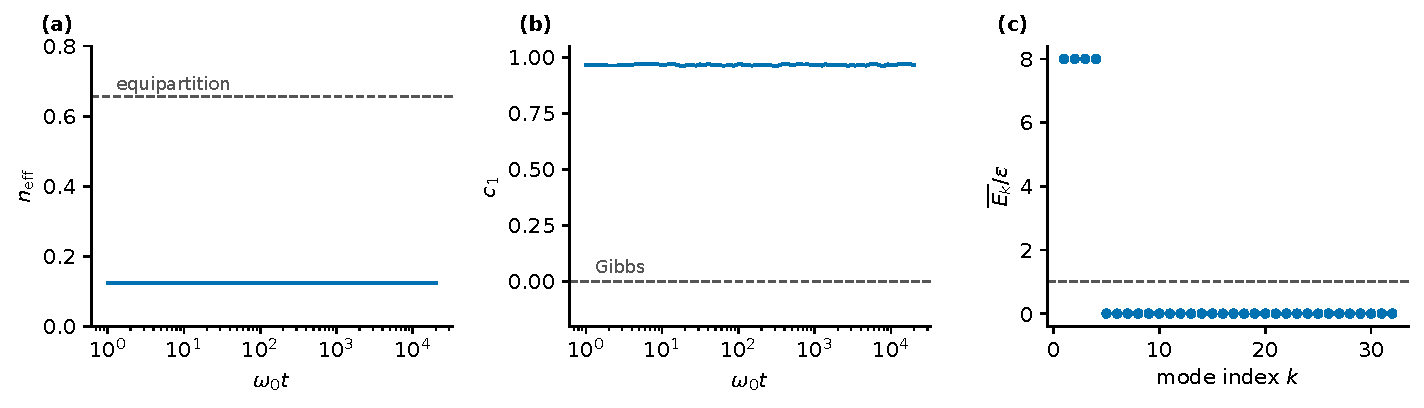
\includegraphics[width=\textwidth]{chain.pdf}
  \caption{Closed harmonic chain ($ N = 32 $, fixed ends, $ \varepsilon = 0.1\,\kappa a^2 $) with the energy initially in the four lowest modes; averages over 16 random initial phases. (a) Effective fraction of excited modes, Eq.~\eqref{eq:neff}; dashed: equipartition value. (b) Nearest-neighbour momentum correlation; dashed: Gibbs value. (c) Mode energies averaged over $ 10^4 < \omega_0 t < 2\times 10^4 $; dashed: equipartition.}
  \label{fig:chain}
\end{figure}

%======================================================================
\section{Harmonic System Weakly Coupled to a Large Bath}
\label{sec:bath}

\subsection{Model}

The system consists of a few coupled harmonic oscillators, with unit masses and mass-weighted coordinates $ x_i $,
\begin{equation}
  H_S = \sum_i \frac{p_i^2}{2} + \frac12 \mathbf x^{\mathsf T} K_S \mathbf x ,
  \qquad
  K_S = U \, \mathrm{diag}(\Omega_a^2) \, U^{\mathsf T} ,
  \label{eq:HS}
\end{equation}
with normal-mode frequencies $ \Omega_a $ and normal coordinates $ Q_a = \sum_i U_{ia} x_i $.
It couples through the coordinate $ x_1 $ to a bath of $ N_B $ harmonic oscillators $ (q_k, p_k) $, written in the Caldeira--Leggett form~\cite{Caldeira1983,Zwanzig1973}
\begin{equation}
  H_B = \sum_{k=1}^{N_B} \bigg[ \frac{p_k^2}{2} + \frac{\omega_k^2}{2} \Big( q_k - \frac{c_k}{\omega_k^2} x_1 \Big)^2 \bigg]
  = \sum_k \Big[ \frac{p_k^2}{2} + \frac{\omega_k^2 q_k^2}{2} \Big] - x_1 \sum_k c_k q_k + \frac{x_1^2}{2} \sum_k \frac{c_k^2}{\omega_k^2} .
  \label{eq:HB}
\end{equation}
The last term (the counter-term) ensures that $ H = H_S + H_B $ is bounded below and that the bath does not shift the static potential of the system.
The bath enters all results only through its spectral density
\begin{equation}
  J(\omega) = \frac{\pi}{2} \sum_k \frac{c_k^2}{\omega_k} \, \delta(\omega - \omega_k) ,
  \label{eq:Jclass}
\end{equation}
which combines the coupling strengths with the density of bath frequencies.
The example used for the numerics is Ohmic, $ J(\omega) = \eta \, \omega $ for $ \omega < \omega_c $; the constant $ \eta $ has units of frequency and is the friction coefficient.

The whole, system plus bath, is a closed harmonic system of the kind treated in Sec.~\ref{sec:chain}.
It does not thermalize as a whole.
The question is whether the system alone does.

\subsection{Exact elimination of the bath}
\label{sec:gle}

The bath equations, $ \ddot q_k = -\omega_k^2 q_k + c_k x_1 $, are linear with a given source $ x_1(t) $, and are solved exactly.
This is the first step of the method and involves no approximation.
Inserting the solution into the force $ \sum_k c_k q_k - x_1 \sum_k c_k^2/\omega_k^2 $ exerted by the bath on $ x_1 $, and integrating by parts once, gives the generalized Langevin equation (GLE)
\begin{equation}
  \ddot x_1(t) = -\frac{\partial V_S}{\partial x_1} - \int_0^t \dd s \, \gamma(t-s) \, \dot x_1(s) + \xi(t) ,
  \label{eq:gle-class}
\end{equation}
with $ V_S = \mathbf x^{\mathsf T} K_S \mathbf x/2 $, the friction kernel and the noise
\begin{align}
  \gamma(t) &= \sum_k \frac{c_k^2}{\omega_k^2} \cos\omega_k t = \frac{2}{\pi} \int_0^\infty \dd\omega \, \frac{J(\omega)}{\omega} \cos\omega t ,
  \label{eq:friction}\\
  \xi(t) &= \sum_k c_k \Big[ \Big( q_k(0) - \frac{c_k}{\omega_k^2} x_1(0) \Big) \cos\omega_k t + \frac{p_k(0)}{\omega_k} \sin\omega_k t \Big] .
  \label{eq:noise}
\end{align}
The other system coordinates obey their Hamiltonian equations unchanged.
If the bath is initially in the Gibbs state at temperature $ T $ for the given $ x_1(0) $, the $ q_k(0) - c_k x_1(0)/\omega_k^2 $ and $ p_k(0) $ are independent Gaussian variables with variances $ \kB T/\omega_k^2 $ and $ \kB T $, and
\begin{equation}
  \langle \xi(t) \rangle = 0 ,
  \qquad
  \langle \xi(t) \, \xi(s) \rangle = \kB T \, \gamma(t-s) .
  \label{eq:fdt-class}
\end{equation}
The noise is Gaussian, and its correlation function is proportional to the friction kernel.
This is the fluctuation--dissipation theorem of the second kind: friction and fluctuations have the same microscopic origin.
For an Ohmic bath with $ \omega_c \to \infty $, $ \gamma(t) = 2\eta\,\delta(t) $ and Eq.~\eqref{eq:gle-class} becomes the ordinary Langevin equation with friction $ \eta $.
Equation~\eqref{eq:gle-class} is an instance of the projection-operator equations of Sec.~\ref{sec:mz-method}; for a harmonic bath the projection can be carried out in closed form~\cite{Zwanzig1973,Zwanzig2001}.

\subsection{Weak-coupling perturbation theory}
\label{sec:averaging}

The GLE is exact but still contains the full memory of the bath.
The second step is perturbation theory in the coupling, organized by the separation of time scales it creates.
The small parameter is the ratio of the relaxation rate $ \Gamma $ (defined below) to the system frequencies $ \Omega_a $ and to their differences $ |\Omega_a - \Omega_b| $.

Introduce the complex amplitude of normal mode $ a $,
\begin{equation}
  \alpha_a = \frac{\Omega_a Q_a + \ii P_a}{\sqrt 2} ,
  \qquad
  E_a = |\alpha_a|^2 ,
  \label{eq:amplitude}
\end{equation}
where $ P_a = \dot Q_a $ and $ E_a $ is the energy of the mode.
Since the bath force acts on $ x_1 = \sum_a u_a Q_a $, with $ u_a \equiv U_{1a} $, the exact equation of motion is $ \dot\alpha_a = -\ii\Omega_a \alpha_a + \ii u_a F(t)/\sqrt 2 $, with $ F $ the sum of the memory and noise terms of Eq.~\eqref{eq:gle-class}.
The slowly varying amplitude $ a_a = \alpha_a e^{\ii\Omega_a t} $ changes only through $ F $.
Its equation is averaged over an interval $ \Delta t $ that is long compared with the bath correlation time $ \tau_B $ (the decay time of $ \gamma $), with $ 1/\Omega_a $ and with $ 1/|\Omega_a - \Omega_b| $, but short compared with $ 1/\Gamma $.
To second order in the couplings $ c_k $ this requires two steps.
\begin{itemize}[leftmargin=1.5em]
\item In the memory term, $ \dot x_1(s) $ is replaced by its unperturbed value, $ \dot x_1(s) = \sum_b u_b P_b(s) $ with $ P_b(s) = -\ii(a_b e^{-\ii\Omega_b s} - a_b^* e^{\ii\Omega_b s})/\sqrt 2 $. After averaging, the terms oscillating at $ \Omega_a \pm \Omega_b $ drop out, except the resonant term $ b = a $ (secular, or rotating-wave, approximation). The upper limit of the memory integral is extended to infinity (Markov approximation), which is justified because $ t \gg \tau_B $.
\item The noise, projected on the rotating frame, $ \eta_a(t) = \ii u_a e^{\ii\Omega_a t} \xi(t)/\sqrt 2 $, is correlated over $ \tau_B \ll \Delta t $ and acts as white noise whose strength is its spectral density at $ \Omega_a $.
\end{itemize}
With $ \hat\gamma(\Omega) = \int_0^\infty \dd\tau \, \gamma(\tau) \, e^{\ii\Omega\tau} $, whose real part is $ \mathrm{Re}\,\hat\gamma(\Omega) = J(\Omega)/\Omega $ by Eq.~\eqref{eq:friction}, the result is the Langevin equation
\begin{equation}
  \dot a_a = -\Big( \frac{\Gamma_a}{2} + \ii\delta_a \Big) a_a + \eta_a(t) ,
  \qquad
  \langle \eta_a(t) \, \eta_b^*(s) \rangle = \delta_{ab} \, \Gamma_a \kB T \, \delta(t-s) ,
  \label{eq:langevin-amp}
\end{equation}
with the energy relaxation rate and the frequency shift
\begin{equation}
  \Gamma_a = u_a^2 \, \frac{J(\Omega_a)}{\Omega_a} ,
  \qquad
  \delta_a = \frac{u_a^2}{2} \, \mathrm{Im}\,\hat\gamma(\Omega_a) .
  \label{eq:gamma-class}
\end{equation}
The rate is second order in the coupling and proportional to the density of bath modes at the system frequency: it is the classical golden rule.
Cross-correlations of the noise between different modes, and the correlation $ \langle \eta_a \eta_a \rangle $, oscillate at $ \Omega_a - \Omega_b $ and $ 2\Omega_a $ and average to zero.

Two results follow from Eq.~\eqref{eq:langevin-amp}.
First, by the It\^o rule $ \dd|a|^2 = a^* \dd a + a \, \dd a^* + |\dd\eta|^2 $, the mean energy obeys $ \dd\langle E_a\rangle/\dd t = -\Gamma_a (\langle E_a\rangle - \kB T) $, so
\begin{equation}
  \langle E_a \rangle(t) = \kB T + \big( E_a(0) - \kB T \big) e^{-\Gamma_a t} .
  \label{eq:Ea-relax}
\end{equation}
Second, writing $ a_a = X + \ii Y $, each of $ X $ and $ Y $ is an Ornstein--Uhlenbeck process~\cite{Risken1989}. Its probability density obeys the Fokker--Planck equation
\begin{equation}
  \partial_t P = \frac{\Gamma_a}{2} \big[ \partial_X (X P) + \partial_Y (Y P) \big] + \frac{\Gamma_a \kB T}{4} \big( \partial_X^2 + \partial_Y^2 \big) P ,
  \label{eq:fokker-planck}
\end{equation}
whose unique stationary solution is $ P \propto \exp[-(X^2 + Y^2)/\kB T] = \exp(-E_a/\kB T) $, approached from any initial density.
Because the noises of different modes are independent, the joint stationary density is $ \prod_a e^{-E_a/\kB T} = e^{-H_S/\kB T} $: the system reaches the Gibbs state at the bath temperature, up to corrections of first order in the coupling.
The modes, which could not exchange energy in isolation (Sec.~\ref{sec:chain}), are now equilibrated with each other through the bath.

The derivation used four conditions, each of which has a physical meaning.
\begin{enumerate}[label=(C\arabic*), leftmargin=3.0em]
\item \label{c:weak} Weak coupling: $ \Gamma_a \ll \Omega_a $ and $ \Gamma_a \ll |\Omega_a - \Omega_b| $.
\item \label{c:markov} Short bath memory: $ \tau_B \ll 1/\Gamma_a $, i.e.\ $ J(\omega)/\omega $ smooth on the scale $ \Gamma_a $ around $ \Omega_a $.
\item \label{c:large} Large bath: the spacing $ \delta\omega $ of bath frequencies is small compared with $ \Gamma_a $, and times are short compared with the bath recurrence time $ 2\pi/\delta\omega $. The energy released by the system, spread over many bath modes, changes the bath temperature only by an amount of order $ 1/N_B $.
\item \label{c:thermal} Thermal bath: the bath is prepared in a Gibbs state.
\end{enumerate}
Condition~\ref{c:thermal} fixes the final state: the noise strength $ \Gamma_a \kB T $ is set by the temperature at which the bath was prepared, so every system mode relaxes to the same $ \kB T $.
The bath imposes its temperature on the system.

\subsection{Numerical test}
\label{sec:bath-numerics}

The perturbative results are tested against the exact solution of the full quadratic Hamiltonian.
The full $ (N_B + 2) $-dimensional stiffness matrix is diagonalized, and Eq.~\eqref{eq:chain-solution} is applied (Appendix~\ref{app:numerics}), so the only errors are statistical.
The system consists of two oscillators of frequency $ \omega_0 $ coupled by a spring of relative stiffness $ 0.3 $, which gives $ \Omega_+ = \omega_0 $, $ \Omega_- = 1.265\,\omega_0 $ and $ u_\pm^2 = 1/2 $.
The bath has $ N_B = 2000 $ modes, an Ohmic density with $ \eta = 0.04\,\omega_0 $ and $ \omega_c = 5\,\omega_0 $, and temperature $ T $.
Equation~\eqref{eq:gamma-class} predicts $ \Gamma_\pm = 0.02\,\omega_0 $.
The four conditions hold: $ \Gamma/(\Omega_- - \Omega_+) = 0.08 $, $ \delta\omega/\Gamma = 0.13 $, and the recurrence time $ 2\pi/\delta\omega \approx 2500/\omega_0 $ exceeds the simulated time eightfold.
The mode $ \Omega_+ $ starts with energy $ 4\kB T $ and the mode $ \Omega_- $ with zero energy; the results are averaged over 4000 realizations of the phases and of the bath.

Figure~\ref{fig:bath}(a) shows that both modes relax to $ \kB T $ as predicted by Eq.~\eqref{eq:Ea-relax}, without adjustable parameters; the largest deviation, $ 0.05\,\kB T $, is within the statistical error.
The late-time distribution of $ E_\pm $ is exponential with mean $ 1.02\,\kB T $ and $ 1.00\,\kB T $ [Fig.~\ref{fig:bath}(b)].
For a small bath, $ N_B = 100 $ with $ \delta\omega = 0.05\,\omega_0 > \Gamma $, condition~\ref{c:large} fails: fewer than one bath mode lies within the linewidth of each system mode, the bath spectrum is discrete on the relevant scale, and the energy oscillates between the system and the few nearly resonant bath modes instead of relaxing [Fig.~\ref{fig:bath}(c)]. The size of the bath, through the spacing of its frequencies, decides whether the system relaxes.

\begin{figure}[t]
  \centering
  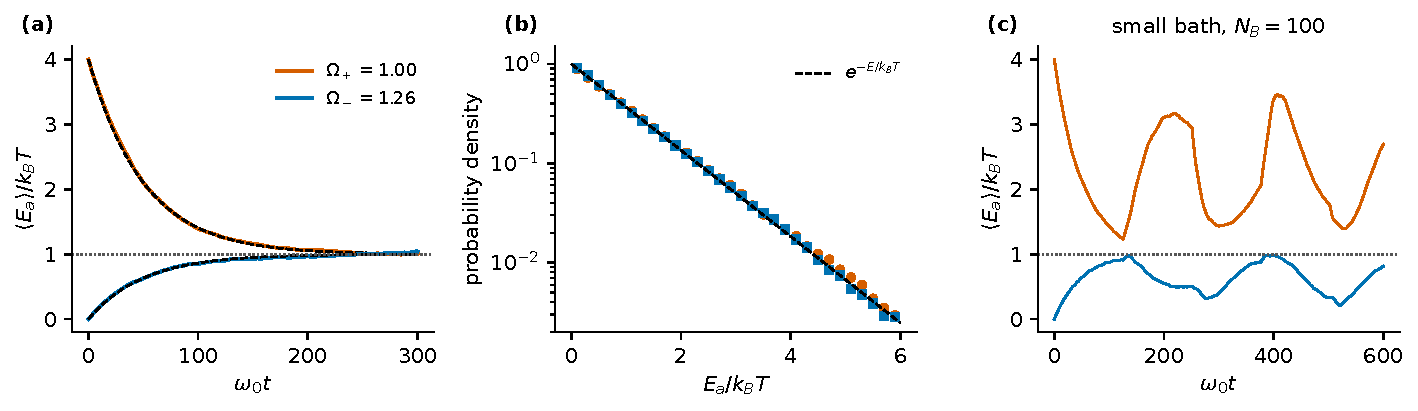
\includegraphics[width=\textwidth]{bath.pdf}
  \caption{Two coupled oscillators coupled to a harmonic bath; exact solution, 4000 realizations. (a) Mean energies of the normal modes $ \Omega_\pm $ for a thermal bath of $ N_B = 2000 $ modes; dashed: Eq.~\eqref{eq:Ea-relax} with the rate~\eqref{eq:gamma-class}. (b) Distribution of the mode energies for $ 200 < \omega_0 t < 300 $; dashed: Gibbs distribution. (c) Small bath, $ N_B = 100 $.}
  \label{fig:bath}
\end{figure}

\subsection{System and bath together}

The relaxation of the system does not make the whole thermal.
The whole is harmonic: its $ N_B + 2 $ normal-mode energies are conserved, and Eq.~\eqref{eq:invariants} holds.
The excess energy $ E_a(0) - \kB T $ of a system mode ends up in the few global normal modes whose frequencies lie within $ \Gamma_a $ of $ \Omega_a $, where it stays; each carries a share of order $ \delta\omega/\Gamma_a $, invisible in any local observable.
By Eq.~\eqref{eq:mutual}, the entropy gained by the system is matched by correlations between system and bath.
In the finite bath of Fig.~\ref{fig:bath}(c) these correlations return to the system within the observation time.
A harmonic system cannot thermalize by itself (Sec.~\ref{sec:chain}); coupled weakly to a large bath prepared at temperature $ T $, it thermalizes at $ T $, while the closed whole does not.

%======================================================================
\section{Quantum System Weakly Coupled to a Bosonic Bath}
\label{sec:quantum}

This section develops the quantum counterpart of Sec.~\ref{sec:bath}.
It shows that the decoherence, the temperature and the entropy of the system are all determined by the two-point correlation function of the bath, and that the temperature enters only through one analytic property of that function.
Units with $ \hbar = \kB = 1 $ are used.

\subsection{Setting and assumptions}

The system with Hamiltonian $ \hat H_S $ and eigenstates $ |n\rangle $ couples to a bath of bosonic modes,
\begin{equation}
  \hat H = \hat H_S + \hat H_B + \hat A \otimes \hat X ,
  \qquad
  \hat H_B = \sum_k \omega_k \hat b_k^\dagger \hat b_k ,
  \qquad
  \hat X = \sum_k g_k \big( \hat b_k + \hat b_k^\dagger \big) ,
  \label{eq:H-quantum}
\end{equation}
where $ \hat A $ is a system operator.
The spectral density $ J(\omega) = \pi \sum_k g_k^2 \, \delta(\omega - \omega_k) $ coincides with Eq.~\eqref{eq:Jclass} when the quantum oscillators of Sec.~\ref{sec:bath} are written as $ q_k = (\hat b_k + \hat b_k^\dagger)/\sqrt{2\omega_k} $, since then $ g_k = c_k/\sqrt{2\omega_k} $.

The bath state $ \hat\rho_B $ is assumed to be stationary and quasi-free.
A state is quasi-free\footnote{Quasi-free is the name used in quantum statistical mechanics; ``Gaussian'' is the common synonym, referring to the Gaussian form of the Wigner function. The property is defined relative to a set of ladder operators: here those of the normal modes of $ \hat H_B $. It is preserved by linear (Bogoliubov) transformations of the modes and destroyed by non-linear ones.} if all its correlation functions of ladder operators follow from the two-point functions by Wick's rule.
For free bosons, the stationary quasi-free states are the products over modes of geometric distributions, $ \hat\rho_B = \prod_k (1 - x_k) \, x_k^{\hat b_k^\dagger \hat b_k} $ with $ x_k = n_k/(1+n_k) $ and arbitrary mean occupations $ n_k $.
Equivalently, $ \hat\rho_B \propto \exp(-\sum_k \lambda_k \omega_k \hat b_k^\dagger \hat b_k) $: a GGE, Eq.~\eqref{eq:gge}, with one multiplier per mode.
It is also the state of maximum entropy for given $ n_k $\footnote{This is Jaynes's maximum-entropy characterization~\cite{Jaynes1957}: maximizing $ -\Tr\hat\rho\ln\hat\rho $ at fixed mean occupations gives the product of geometric distributions; at fixed mean energy it gives $ e^{-\beta \hat H_B}/Z $, with $ \beta $ the Lagrange multiplier. The principle selects a state; it does not explain why a physical bath is found in it.}.
The Gibbs state is the special case $ \lambda_k = \beta $ for all $ k $, i.e.\ $ n_k = n_{\mathrm B}(\omega_k) = 1/(e^{\beta\omega_k} - 1) $.
A mode in a number (Fock) state is not quasi-free.
For a large bath in which no single mode dominates $ \hat X $ ($ g_k^2 = O(1/N_B) $), $ \hat X $ is a sum of many independent contributions and has Gaussian statistics by the central limit theorem, even without the quasi-free assumption.

Two further assumptions, the same as in Sec.~\ref{sec:bath}, control the analysis:
\begin{itemize}[leftmargin=1.5em]
\item the bath is large, so that its spectrum is continuous on the scale of the relaxation rates and the change of each mode caused by the system is of order $ 1/N_B $;
\item the coupling is weak compared with the bandwidth of the bath and with the spacings of the Bohr frequencies $ \omega_{nm} = E_n - E_m $ of the system.
\end{itemize}
Neither assumption requires the bath to be thermal.

Two methods are used, each where it is exact or controlled.
For a coupling that commutes with $ \hat H_S $, the dynamics is solved exactly with the Wick identity (Sec.~\ref{sec:dephasing}).
For a general coupling, the reduced dynamics is obtained to second order in the coupling (Born--Markov--secular approximation, Sec.~\ref{sec:master}), which becomes exact in the weak-coupling limit~\cite{Davies1974}.

\subsection{Wick identity}

For an operator $ \hat X $ linear in the ladder operators and a quasi-free state with $ \langle\hat X\rangle = 0 $,
\begin{equation}
  \big\langle e^{\ii\hat X} \big\rangle = \exp\Big( -\frac12 \langle \hat X^2 \rangle \Big) .
  \label{eq:wick}
\end{equation}
Wick's rule gives $ \langle \hat X^{2k} \rangle = (2k-1)!! \, \langle \hat X^2 \rangle^k $: there are $ (2k-1)!! $ ways to pair $ 2k $ factors, and all pairings give the same value because $ \hat X $ commutes with itself.
Summing the exponential series, $ \sum_k (-1)^k (2k-1)!! \langle\hat X^2\rangle^k/(2k)! = \sum_k (-\langle\hat X^2\rangle/2)^k/k! $.
Equation~\eqref{eq:wick} is the operator form of the statement that the average of an exponential is the exponential of the connected (cumulant) average, and that for Gaussian statistics only the second cumulant survives.
It requires neither a temperature nor a Gibbs state; for the vacuum, $ \langle\hat X^2\rangle $ is the zero-point fluctuation.

\subsection{Decoherence without energy exchange; the Debye--Waller factor}
\label{sec:dephasing}

Let the coupling commute with $ \hat H_S $, $ \hat A |\mu\rangle = a_\mu |\mu\rangle $ (pure dephasing).
Each system state $ |\mu\rangle $ then drives the bath with its own Hamiltonian $ \hat H_B + a_\mu \hat X $ and evolution operator $ \hat U_\mu(t) $, and the reduced density matrix is exactly
\begin{equation}
  \rho_{\mu\nu}(t) = \rho_{\mu\nu}(0) \, e^{-\ii(E_\mu - E_\nu)t} \, \big\langle \hat U_\nu^\dagger(t) \hat U_\mu(t) \big\rangle_B ,
  \label{eq:dephasing}
\end{equation}
where the partial trace over the bath has become an ordinary bath expectation value by cyclicity of the trace.
Since $ \hat X $ is linear in the modes, $ \hat U_\nu^\dagger \hat U_\mu $ is, up to a phase, a displacement operator: the exponential of a linear combination of ladder operators.
Equation~\eqref{eq:wick} then gives
\begin{equation}
  \begin{gathered}
  \big| \big\langle \hat U_\nu^\dagger(t) \hat U_\mu(t) \big\rangle \big|
  = \exp\big[ -(a_\mu - a_\nu)^2 \, \Phi(t) \big] ,
  \\
  \Phi(t) = \int_0^\infty \frac{\dd\omega}{\pi} \, J(\omega) \, \big[ 2n(\omega) + 1 \big] \, \frac{1 - \cos\omega t}{\omega^2} ,
  \end{gathered}
  \label{eq:decoherence}
\end{equation}
the decoherence function of the independent-boson model~\cite{Mahan2000,Breuer2002}, with $ n(\omega) $ the mode occupation ($ 2n+1 = \coth(\beta\omega/2) $ for a thermal bath).
The populations $ \rho_{\mu\mu} $ do not change: no energy is exchanged, yet the coherences decay.
For an Ohmic bath at $ T > 0 $, $ \Phi(t) \simeq \eta T t $ at long times, and coherences decay exponentially.
For a super-Ohmic bath at $ T = 0 $, $ \Phi(\infty) $ is finite and coherence saturates at a non-zero plateau.

The Debye--Waller factor is the instantaneous version of Eq.~\eqref{eq:dephasing}.
A probe (a neutron, an X-ray photon or a $ \gamma $-ray) that transfers momentum $ \mathbf q $ to a nucleus with displacement $ \hat{\mathbf u} $ acts on the lattice with $ \hat U_{\mathbf q} = e^{\ii \mathbf q \cdot \hat{\mathbf u}} $.
For a probe in a superposition of two momentum transfers, Eq.~\eqref{eq:wick} gives
\begin{equation}
  \langle \hat U_{\mathbf q_2}^\dagger \hat U_{\mathbf q_1} \rangle = e^{-W(\mathbf q_1 - \mathbf q_2)} ,
  \qquad
  W(\mathbf q) = \tfrac12 \big\langle (\mathbf q \cdot \hat{\mathbf u})^2 \big\rangle .
  \label{eq:debye-waller}
\end{equation}
The Debye--Waller exponent is thus the decoherence exponent of the probe; the attenuation of Bragg intensities, $ e^{-2W} $, is its measurable form.
For equal weights of the two branches, the reduced density matrix of the probe has eigenvalues $ \lambda_\pm = (1 \pm e^{-W})/2 $, and its von Neumann entropy
\begin{equation}
  S_{\mathrm{ent}} = -\lambda_+ \ln\lambda_+ - \lambda_- \ln\lambda_-
  \label{eq:S-ent}
\end{equation}
is non-zero already at $ T = 0 $, where $ W $ is set by the zero-point motion.
If the global state is pure, as for a lattice in its ground state, $ S_{\mathrm{ent}} $ is the entanglement entropy between probe and lattice.
The entropy of the probe originates in entanglement with the bath; a temperature only increases it.

\subsection{Temperature as the detailed-balance parameter of the bath}
\label{sec:kms}

Temperature enters through the bath correlation functions
\begin{equation}
  C^>(t) = \langle \hat X(t) \hat X(0) \rangle_B ,
  \qquad
  C^<(t) = \langle \hat X(0) \hat X(t) \rangle_B ,
  \qquad
  C^\gtrless(\omega) = \int \dd t \, e^{\ii\omega t} C^\gtrless(t) ,
  \label{eq:bath-corr}
\end{equation}
with $ \hat X(t) = e^{\ii\hat H_B t} \hat X e^{-\ii\hat H_B t} $.
$ C^>(\omega) $ is the spectral density of transitions in which the bath absorbs energy $ \omega $, and $ C^<(\omega) = C^>(-\omega) $ that of transitions in which it emits $ \omega $.
For the Gibbs state, cyclicity of the trace gives the Kubo--Martin--Schwinger (KMS) condition
\begin{equation}
  C^>(t) = C^<(t + \ii\beta)
  \qquad\Longleftrightarrow\qquad
  C^>(\omega) = e^{\beta\omega} \, C^<(\omega) ,
  \label{eq:kms}
\end{equation}
the second form being detailed balance.
With the symmetrized fluctuation $ S_X = (C^> + C^<)/2 $ and the dissipative response $ \chi_X'' = (C^> - C^<)/2 $ (positive for $ \omega > 0 $), Eq.~\eqref{eq:kms} is equivalent to the fluctuation--dissipation theorem
\begin{equation}
  S_X(\omega) = \coth\frac{\beta\omega}{2} \; \chi_X''(\omega) ,
  \qquad
  \coth\frac{\beta\omega}{2} = 1 + 2 n_{\mathrm B}(\omega) .
  \label{eq:fdt}
\end{equation}
For the free bath, $ C^>(\omega) = 2J(\omega)[1 + n(\omega)] $ and $ C^<(\omega) = 2J(\omega)\, n(\omega) $ for $ \omega > 0 $, so the ratio $ C^>/C^< = (1+n)/n $ equals $ e^{\beta\omega} $ at every frequency only if $ n(\omega) = n_{\mathrm B}(\omega) $.
Temperature is therefore a property of the bath correlation function, the parameter of its detailed-balance relation.
In the Debye--Waller exponent, $ W = \frac12 \int \frac{\dd\omega}{2\pi} S_X(\omega) $, it appears only through the factor $ \coth(\beta\omega/2) $.

\subsection{Relaxation: golden-rule rates and the Gibbs state}
\label{sec:master}

For a coupling that does not commute with $ \hat H_S $, the method is second-order perturbation theory for the reduced density matrix $ \hat\rho_S = \Tr_B \hat\rho $.
In the interaction picture, integrating the von Neumann equation twice and tracing over the bath gives, since $ \langle\hat X\rangle = 0 $,
\begin{equation}
  \frac{\dd\tilde\rho_S}{\dd t} = -\int_0^t \dd s \, \Tr_B \big[ \tilde V(t), [\tilde V(s), \tilde\rho(s)] \big] .
  \label{eq:born-exact}
\end{equation}
Three approximations, each tied to one of the assumptions above, reduce it to a closed equation.
\begin{itemize}[leftmargin=1.5em]
\item Born: $ \tilde\rho(s) \simeq \tilde\rho_S(s) \otimes \hat\rho_B $. The bath is large, so the system changes each bath mode only at order $ 1/N_B $.
\item Markov: $ \tilde\rho_S(s) \to \tilde\rho_S(t) $ and $ \int_0^t \to \int_0^\infty $. The bath correlation time $ \tau_B $ is short compared with the relaxation time.
\item Secular: terms oscillating at differences of Bohr frequencies are dropped. The relaxation rates are small compared with those differences.
\end{itemize}
For a non-degenerate spectrum the populations $ P_n = \langle n | \hat\rho_S | n \rangle $ then obey the Pauli master equation~\cite{Pauli1928,vanHove1955,Breuer2002}
\begin{equation}
  \frac{\dd P_n}{\dd t} = \sum_m \big[ W_{nm} P_m - W_{mn} P_n \big] ,
  \qquad
  W_{mn} = |A_{mn}|^2 \, C^>(E_n - E_m) ,
  \label{eq:pauli}
\end{equation}
where $ W_{mn} $ is the golden-rule rate from $ |n\rangle $ to $ |m\rangle $: the squared matrix element times the ability of the bath to absorb the energy $ E_n - E_m $.
The coherences decay at the rates $ (\Gamma_n + \Gamma_m)/2 $, with $ \Gamma_n = \sum_{m\neq n} W_{mn} $, plus the pure-dephasing contribution of Sec.~\ref{sec:dephasing}.
Davies proved that these equations become exact in the weak-coupling limit, in which the coupling $ \lambda \to 0 $ at fixed $ \lambda^2 t $~\cite{Davies1974}.

Detailed balance of the bath carries over to the rates.
With $ \omega = E_n - E_m $, Eq.~\eqref{eq:kms} gives
\begin{equation}
  \frac{W_{mn}}{W_{nm}} = \frac{C^>(\omega)}{C^>(-\omega)} = \frac{C^>(\omega)}{C^<(\omega)} = e^{\beta (E_n - E_m)} ,
  \label{eq:detailed-balance}
\end{equation}
so $ \pi_n = e^{-\beta E_n}/Z_S $ is a stationary solution with every pair of transitions balanced, and it is the only one if the rates connect all levels.
Relaxation to it is monotonic: with $ x_n = P_n/\pi_n $ and the symmetric weights $ w_{nm} = W_{nm}\pi_m $,
\begin{equation}
  \frac{\dd}{\dd t} D(P \Vert \pi) = -\frac12 \sum_{n,m} w_{nm} \, (x_m - x_n)(\ln x_m - \ln x_n) \le 0 ,
  \label{eq:h-theorem}
\end{equation}
the $ H $-theorem of the master equation; Spohn's theorem extends it to the full quantum dynamical semigroup~\cite{Spohn1978}.
The irreversibility enters through the Born and Markov steps, which discard the system--bath correlations, and through the initial product state, which fixes the direction of time.
The structure is that of Boltzmann's kinetic theory, with the golden-rule rates as collision integral and the Born factorization as the counterpart of the molecular-chaos assumption.

For a harmonic oscillator, $ \hat A = (\hat a + \hat a^\dagger)/\sqrt{2\Omega} $, Eq.~\eqref{eq:pauli} gives $ \dd\langle \hat a^\dagger \hat a\rangle/\dd t = -[J(\Omega)/\Omega] \, (\langle \hat a^\dagger\hat a\rangle - n(\Omega)) $: the rate of Eq.~\eqref{eq:gamma-class} with $ u_a = 1 $, and the classical result in the limit $ n \to \kB T/\Omega $.

\subsection{Thermality test: generalized fluctuation--dissipation relations}
\label{sec:gen-fdt}

The stationary populations are only one test of thermality.
A stricter test uses the correlation functions of any system observable $ \hat O $ in the stationary state and defines a frequency-dependent inverse temperature by
\begin{equation}
  S_O(\omega) \equiv \coth\frac{\beta_{\mathrm{eff}}(\omega)\,\omega}{2} \; \chi_O''(\omega) ,
  \label{eq:beta-eff}
\end{equation}
i.e.\ by the measured ratio of fluctuation to dissipation at each frequency.
Equation~\eqref{eq:beta-eff} is a definition; the system is thermal in the operational sense if $ \beta_{\mathrm{eff}} $ is the same constant for all frequencies and all observables.
In the weak-coupling limit with a thermal bath this holds: the generator of the Davies limit satisfies quantum detailed balance with respect to the Gibbs state, and stationary correlation functions computed from it by the quantum regression theorem obey the KMS relation with the bath's $ \beta $~\cite{Davies1974,Breuer2002}.
The criterion fails, informatively, in two situations.
\begin{enumerate}[label=(\roman*), leftmargin=2.2em]
\item Strong coupling. The reduced equilibrium state is $ \Tr_B e^{-\beta\hat H}/Z \equiv e^{-\beta \hat H_S^*}/Z^* $, which defines the Hamiltonian of mean force $ \hat H_S^* $; it differs from $ \hat H_S $ at first order in the coupling and depends on $ \beta $. The system is thermal with respect to $ \hat H_S^* $, not $ \hat H_S $.
\item Glassy or driven systems. The ratio defines different effective temperatures on different time scales~\cite{Cugliandolo2011}.
\end{enumerate}

\subsection{Fermionic bath}
\label{sec:fermionic}

Three differences arise when the bath is a Fermi sea of conduction electrons.
First, physical couplings contain an even number of fermion operators (fermion-parity superselection\footnote{Superselection rule: no physical observable connects states of even and odd fermion number, so every term of a Hamiltonian contains an even number of fermion operators.}), so the lowest coupling is a bilinear, $ \hat X = \sum_{kk'} g_{kk'} \hat c_k^\dagger \hat c_{k'} $. The bath excitations are then particle--hole pairs, whose density of states at low energy transfer $ \omega $ grows as $ \omega $: the bath is Ohmic.
Second, the KMS condition~\eqref{eq:kms} holds for the even operator $ \hat X $, so the Gibbs state is reached as before, but the rates contain the Pauli factor $ f(\epsilon)[1 - f(\epsilon + \omega)] $. For level splittings $ \omega \ll T $ this gives the Korringa law $ 1/T_1 \propto (g \nu_F)^2 \, T $, with $ \nu_F $ the density of states at the Fermi energy~\cite{Korringa1950}.
Third, Eq.~\eqref{eq:wick} does not apply, because $ \hat X $ is quadratic in the fermion operators. The overlap between the Fermi sea and the Fermi sea in the presence of a local potential with phase shift $ \delta $ vanishes as $ N^{-(\delta/\pi)^2} $ (Anderson's orthogonality catastrophe~\cite{Anderson1967}), and at $ T = 0 $ coherence decays as $ t^{-(\delta/\pi)^2} $~\cite{Nozieres1969}. No coherence plateau analogous to the Debye--Waller factor exists for a Fermi sea.

\subsection{Quantitative example: Debye phonon bath}
\label{sec:debye}

For a Debye model, with density of states $ g(\omega) = 9N\omega^2/\omega_D^3 $ below the Debye frequency $ \omega_D = \Theta_D $, the isotropic exponent of Eq.~\eqref{eq:debye-waller} for a nucleus of mass $ M $ is
\begin{equation}
  W(\mathbf q, T) = \frac{3 q^2}{4 M \omega_D} \, \Phi(T/\Theta_D) ,
  \qquad
  \Phi(x) = \int_0^1 \dd u \, u \coth\frac{u}{2x} ,
  \label{eq:W-debye}
\end{equation}
with the limits
\begin{equation}
  W \simeq
  \begin{cases}
    W_0 \Big[ 1 + \dfrac{2\pi^2}{3} \Big( \dfrac{T}{\Theta_D} \Big)^2 \Big] , & T \ll \Theta_D , \\[8pt]
    4 W_0 \, T/\Theta_D , & T \gg \Theta_D ,
  \end{cases}
  \qquad
  W_0 = \frac{3 q^2}{8 M \omega_D} .
  \label{eq:W-limits}
\end{equation}
The entanglement entropy~\eqref{eq:S-ent} with $ W = W(\mathbf q_1 - \mathbf q_2, T) $ behaves as $ (W_0/2)[1 - \ln(W_0/2)] $ for $ W_0 \ll 1 $ at $ T = 0 $, and approaches $ \ln 2 - e^{-2W}/2 $ at high temperature (Fig.~\ref{fig:debye}).
The thermodynamic entropy of the lattice, $ S_{\mathrm{th}} = \int \dd\omega \, g(\omega)[(1+n_{\mathrm B})\ln(1+n_{\mathrm B}) - n_{\mathrm B}\ln n_{\mathrm B}] $, grows as $ (4\pi^4/5) N (T/\Theta_D)^3 $ at low and as $ 3N[\ln(T/\Theta_D) + 4/3] $ at high temperature.
The two entropies are different quantities.
$ S_{\mathrm{ent}} $, the entropy of a two-branch probe, is bounded by $ \ln 2 $; $ S_{\mathrm{th}} $ is extensive.
What they share is the phonon spectrum $ g(\omega) $ weighted by the occupations.
A measurement of $ W(T) $, through Bragg or M\"ossbauer intensities or interferometric visibility, determines $ g(\omega) $, which in turn predicts $ S_{\mathrm{th}}(T) $; this is a consistency test linking single-probe decoherence to bulk thermodynamics.

\begin{figure}[t]
  \centering
  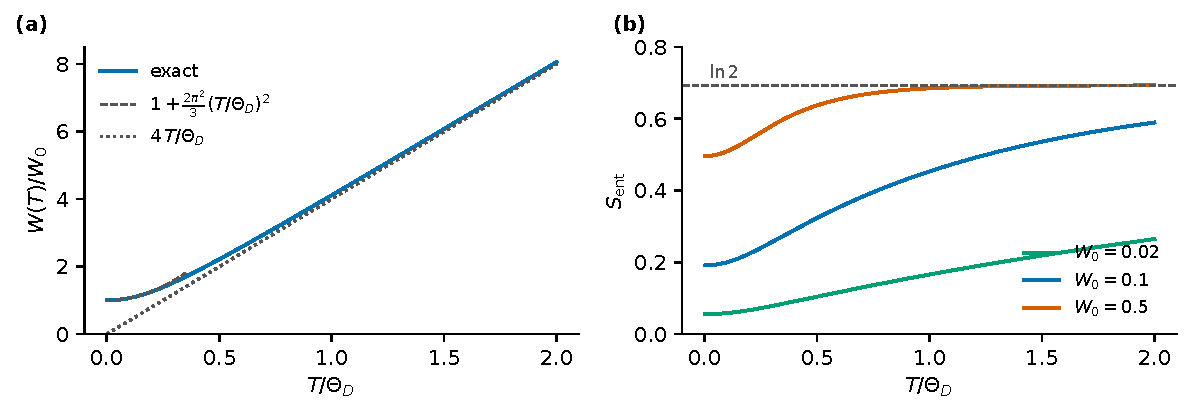
\includegraphics[width=0.78\textwidth]{debye.pdf}
  \caption{Debye bath. (a) Debye--Waller exponent, Eq.~\eqref{eq:W-debye}, with its low- and high-temperature limits, Eq.~\eqref{eq:W-limits}. (b) Entanglement entropy of a probe in an equal-weight superposition of two momentum transfers, Eq.~\eqref{eq:S-ent}, for three values of the zero-point exponent $ W_0 $.}
  \label{fig:debye}
\end{figure}

\subsection{Scope}

The construction takes the state of the bath as given.
It shows that a weakly coupled system inherits the temperature of that state: if the bath obeys detailed balance at $ \beta $, the system relaxes to its Gibbs state at $ \beta $, with its thermodynamic entropy.
Two questions are left open.
First, why a physical bath is found in a thermal state: canonical typicality~\cite{Goldstein2006,Popescu2006} and the eigenstate thermalization hypothesis~\cite{Deutsch1991,Srednicki1994,Rigol2008,DAlessio2016} (Appendix~\ref{app:eth}) address this for closed systems, and Sec.~\ref{sec:mz} examines a closed system in which the bath is internal.
Second, what happens to the whole: the global state remains pure if it started pure, and the system entropy is matched, by Eq.~\eqref{eq:mutual}, by system--bath correlations.

%======================================================================
\section{Slow and Fast Modes in an Isolated Bose Gas: Mori--Zwanzig Analysis}
\label{sec:mz}

\subsection{The Mori--Zwanzig projection method}
\label{sec:mz-method}

In Secs.~\ref{sec:bath} and~\ref{sec:quantum} the system and the bath were given.
In a closed system without an external bath, one must first decide which variables are the ``system''.
The projection-operator method of Mori and Zwanzig~\cite{Nakajima1958,Zwanzig1960,Zwanzig1961,Mori1965} makes this decision explicit.
One chooses a set of relevant variables, and the method rewrites the exact equations of motion for them as a generalized Langevin equation, in which all other degrees of freedom of the same closed system act as a bath through a memory kernel and a fluctuating force.
The rewriting is exact; irreversibility appears only when the memory kernel decays, and a simple (Markovian) description only when it decays fast.
The presentation follows Refs.~\cite{Forster1975,Zwanzig2001,Grabert1982}.

\paragraph{Liouvillian.}
The time evolution of an observable $ A $ is generated by the Liouville operator $ \LL $,
\begin{equation}
  \frac{\dd A}{\dd t} = \ii \LL A ,
  \qquad
  A(t) = e^{\ii\LL t} A ,
  \qquad
  \ii\LL A =
  \begin{cases}
    \{ A , H \} & \text{(classical)} , \\
    \ii [ \hat H , \hat A ] & \text{(quantum, } \hbar = 1 \text{)} .
  \end{cases}
  \label{eq:liouvillian}
\end{equation}
$ \LL $ acts on the linear space of observables, just as $ \hat H $ acts on the space of state vectors.

\paragraph{Scalar product.}
Observables are treated as vectors with the Kubo scalar product in the equilibrium state $ \hat\rho_{\mathrm{eq}} = e^{-\beta\hat H}/Z $,
\begin{equation}
  \sprod{A}{B} = \frac{1}{\beta} \int_0^\beta \dd\lambda \, \big\langle e^{\lambda\hat H} \hat A^\dagger e^{-\lambda\hat H} \hat B \big\rangle_{\mathrm{eq}} - \langle \hat A^\dagger \rangle_{\mathrm{eq}} \langle \hat B \rangle_{\mathrm{eq}} ,
  \label{eq:kubo}
\end{equation}
which reduces to the covariance $ \langle \delta A^* \, \delta B \rangle_{\mathrm{eq}} $ in classical mechanics.
It is positive, $ \sprod{A}{A} \ge 0 $, and $ \LL $ is Hermitian with respect to it, $ \sprod{A}{\LL B} = \sprod{\LL A}{B} $; both follow from cyclicity of the trace and $ [\hat\rho_{\mathrm{eq}}, \hat H] = 0 $ (classically, from integration by parts).
Hence $ e^{\ii\LL t} $ is unitary.
The Kubo product is chosen because of its physical meaning.
If a static field $ h $ conjugate to $ \hat A $ acts until $ t = 0 $ ($ \hat H \to \hat H - h\hat A $) and is then switched off, linear-response theory gives exactly~\cite{Kubo1957}
\begin{equation}
  \frac{\delta\langle \hat A \rangle(t)}{\delta\langle \hat A \rangle(0)} = \frac{C(t)}{C(0)} ,
  \qquad
  C(t) = \sprod{A}{A(t)} ,
  \label{eq:relaxation-function}
\end{equation}
and $ \beta C(0) $ is the static susceptibility.
The correlation function $ C(t) $ is therefore the relaxation of a small non-equilibrium deviation, the quantity that thermalization is about.

\paragraph{Projector.}
For relevant variables $ A_1, \dots, A_n $ with static correlation matrix $ \chi_{ij} = \sprod{A_i}{A_j} $, the operator
\begin{equation}
  \PP X = \sum_{j,l} A_j \, (\chi^{-1})_{jl} \, \sprod{A_l}{X} ,
  \qquad
  \QQ = 1 - \PP ,
  \label{eq:projector}
\end{equation}
is the orthogonal projection onto their linear span.
It satisfies $ \PP^2 = \PP $ and $ \PP A_i = A_i $, and it is Hermitian.
$ \PP X $ is the best linear estimate of $ X $ in terms of the $ A_i $, and $ \QQ X $ is the part of $ X $ uncorrelated with all of them.
The $ \QQ $ space is the bath of the formalism: every degree of freedom not represented by the relevant variables.

\paragraph{Operator identity.}
The derivation rests on the identity
\begin{equation}
  e^{\ii\LL t} = e^{\ii\QQ\LL t} + \int_0^t \dd s \, e^{\ii\LL(t-s)} \, \PP \ii\LL \, e^{\ii\QQ\LL s} ,
  \label{eq:dyson}
\end{equation}
which follows by integrating from $ 0 $ to $ t $ the derivative of $ f(s) = e^{\ii\LL(t-s)} e^{\ii\QQ\LL s} $,
\begin{equation*}
  f'(s) = e^{\ii\LL(t-s)} \big( -\ii\LL + \ii\QQ\LL \big) e^{\ii\QQ\LL s} = -e^{\ii\LL(t-s)} \, \PP \ii\LL \, e^{\ii\QQ\LL s} .
\end{equation*}
It separates the full evolution into the evolution confined to the $ \QQ $ space and the returns to the relevant subspace.

\paragraph{Generalized Langevin equation.}
Split the time derivative as $ \dot A_i(t) = e^{\ii\LL t} (\PP + \QQ) \ii\LL A_i $.
The $ \PP $ part is a linear combination of the $ A_j(t) $.
To the $ \QQ $ part, apply Eq.~\eqref{eq:dyson}.
Because $ \ii\LL $ is anti-Hermitian and $ F_i(s) $ lies in the $ \QQ $ space, $ \sprod{A_l}{\ii\LL F_i(s)} = -\sprod{\QQ\ii\LL A_l}{F_i(s)} = -\sprod{F_l}{F_i(s)} $, which turns the returning term into a memory integral.
The result is exact:
\begin{equation}
  \boxed{
  \frac{\dd A_i(t)}{\dd t}
  = \sum_j \ii\Omega_{ij} \, A_j(t)
  - \sum_j \int_0^t \dd s \, K_{ij}(s) \, A_j(t-s)
  + F_i(t)
  }
  \label{eq:gle}
\end{equation}
with
\begin{align}
  \ii\Omega_{ij} &= \sum_l \sprod{A_l}{\ii\LL A_i} (\chi^{-1})_{lj}
  && \text{(frequency matrix)},
  \label{eq:omega}\\
  F_i(t) &= e^{\ii\QQ\LL t} \, \QQ \ii\LL A_i
  && \text{(fluctuating force)},
  \label{eq:force}\\
  K_{ij}(t) &= \sum_l \sprod{F_l}{F_i(t)} (\chi^{-1})_{lj}
  && \text{(memory kernel)}.
  \label{eq:kernel}
\end{align}
The frequency term describes the instantaneous, reversible motion within the relevant subspace.
The fluctuating force is the part of $ \dot A_i $ that cannot be expressed through the relevant variables; it evolves in the $ \QQ $ space and remains uncorrelated with them, $ \sprod{A_j}{F_i(t)} = 0 $ for all $ t $.
The memory kernel is the autocorrelation of the fluctuating force (the fluctuation--dissipation theorem of the second kind~\cite{Kubo1966}), exactly as $ \gamma(t) $ is the noise correlation in Eq.~\eqref{eq:fdt-class}.
For the harmonic bath of Sec.~\ref{sec:bath}, the $ \QQ $ space is the bath and Eq.~\eqref{eq:gle} is Eq.~\eqref{eq:gle-class}.

Taking the scalar product of Eq.~\eqref{eq:gle} with $ A_k $ removes the fluctuating force and gives a closed equation for the correlation matrix $ C_{ij}(t) = \sprod{A_j}{A_i(t)} $,
\begin{equation}
  \dot C(t) = \ii\Omega \, C(t) - \int_0^t \dd s \, K(s) \, C(t-s) ,
  \qquad
  \tilde C(z) = \big[ z - \ii\Omega + \tilde K(z) \big]^{-1} \chi ,
  \label{eq:corr-eq}
\end{equation}
with the Laplace transform $ \tilde f(z) = \int_0^\infty \dd t \, e^{-zt} f(t) $.
For a single Hermitian variable of definite time-reversal parity, $ \Omega = 0 $.

\paragraph{Exactness.}
Equation~\eqref{eq:gle} contains exactly the information of the microscopic equations and is time-reversal symmetric, since $ C(-t) = C(t) $ for such a variable.
Nothing has been approximated; in particular, no information has been discarded.
Irreversible decay of $ C(t) $ requires the memory kernel to decay, and the physical question is how a kernel can decay in a closed system that cannot dissipate information.

\paragraph{How a memory kernel decays in a closed system.}
$ K(t) $ is a correlation function of the projected dynamics $ \QQ\LL\QQ $.
In a finite quantum system, or any system with a discrete spectrum, it has the form
\begin{equation}
  K(t) = \sum_{\alpha} w_\alpha \cos \nu_\alpha t ,
  \qquad
  \overline{K^2} = \frac12 \sum_{\alpha} w_\alpha^2 > 0 ,
  \label{eq:kernel-sum}
\end{equation}
with weights $ w_\alpha $ and frequencies $ \nu_\alpha $ given by the eigenvalues of $ \QQ\LL\QQ $, and $ \overline{\cdots} $ the infinite-time average (written for non-degenerate, non-zero frequencies).
Such an almost-periodic function cannot decay for ever: its mean square is non-zero, and it returns arbitrarily close to its initial value.
It can, however, decay for all practical purposes, by dephasing.
Suppose the weight is spread over $ M_{\mathrm{eff}} = (\sum_\alpha w_\alpha)^2 / \sum_\alpha w_\alpha^2 \gg 1 $ frequencies with spread $ \sigma_\nu $, and the frequencies are non-degenerate and incommensurate.
Then the terms of Eq.~\eqref{eq:kernel-sum} lose their phase relation after a time $ \tau_c \sim 1/\sigma_\nu $, and $ K(t) $ falls from $ K(0) $ to fluctuations of relative size $ M_{\mathrm{eff}}^{-1/2} $.
It stays there until the phases realign, which takes at least the inverse spacing of neighbouring frequencies and, for incommensurate frequencies, a time that grows exponentially with $ M_{\mathrm{eff}} $.
A strictly continuous spectrum is the limit $ M_{\mathrm{eff}} \to \infty $ of this mechanism, not a requirement for it.

No information is lost in the process.
It is moved into phase relations between the relevant variables and a large number of $ \QQ $-space components, which no relevant observable can read.
Reversing all velocities (an echo experiment) would restore it.
The mechanism is the same as the decoherence of Sec.~\ref{sec:dephasing}, where $ \Phi(t) $ grows because the bath frequencies dephase, and as the damping of Sec.~\ref{sec:bath}, where the $ \approx \Gamma_a/\delta\omega $ bath modes within a linewidth play the role of the $ M_{\mathrm{eff}} $ frequencies.
It has two requirements.
\begin{itemize}[leftmargin=1.5em]
\item A large $ \QQ $ space. The decisive parameter is the size of the bath, internal or external. The spacing of the frequencies decreases with size: $ \delta\omega \propto 1/N_B $ for a bath of $ N_B $ modes, and the mean level spacing is $ \sim W/D $ for a many-body spectrum of width $ W $ and Hilbert-space dimension $ D $. On times $ t \ll 1/\delta\omega $ the spectrum cannot be distinguished from a continuum, and $ M_{\mathrm{eff}} $ grows with the size. A small system has well-separated levels, few effective frequencies, and a kernel that returns quickly.
\item Non-degenerate, incommensurate frequencies. In non-integrable systems level repulsion (Appendix~\ref{app:integrability}) removes degeneracies. In integrable systems the conserved quantities put weight at zero frequency (Mazur's bound, below) and make frequencies commensurate, so the kernel does not decay; the harmonic chain of Sec.~\ref{sec:chain} is the extreme case.
\end{itemize}
In classical mechanics a further route exists: in a mixing\footnote{A dynamical system is mixing if the correlation of any two phase-space functions decays to the product of their averages. Mixing implies ergodicity, but not conversely.} (chaotic) system the Liouvillian has a continuous spectrum even with few degrees of freedom. Correlations of smooth observables decay because phase-space densities are stretched into ever finer filaments, and the information moves to scales that smooth observables do not resolve. Quantum mechanics stops this at the scale of $ \hbar $, after which the mechanism above takes over.
In a finite system the residual $ M_{\mathrm{eff}}^{-1/2} $ is a finite-size memory of the initial state; Sec.~\ref{sec:lenk-mz} measures it.

\paragraph{Definition of slow and fast variables.}
Suppose $ K(t) $ has decayed after a time $ \tau_c $, the correlation time of the $ \QQ $ space, and the dissipative part of the dynamics of the relevant variables is slow on this scale.
Then $ C(t-s) \simeq C(t) $ over the range of the kernel, up to the reversible oscillation generated by $ \Omega $, and Eq.~\eqref{eq:corr-eq} becomes
\begin{equation}
  C(t) \simeq e^{(\ii\Omega - \Gamma) t} \, \chi ,
  \qquad
  \Gamma = \tilde K(0) = \int_0^\infty \dd t \, K(t) ,
  \label{eq:markov}
\end{equation}
for non-oscillating variables ($ \Omega = 0 $); for oscillating ones, $ \tilde K $ is evaluated at their frequencies.
This Markov limit is the step at which the exact, reversible equation becomes an irreversible one.
$ K(0) = \sprod{\QQ\LL A}{\QQ\LL A}/\sprod{A}{A} $ is the mean-square coupling of $ A $ to the $ \QQ $ space, and $ \Gamma \approx K(0)\,\tau_c $ is coupling squared times correlation time, the structure of the golden rule.
The limit is consistent if
\begin{equation}
  \varepsilon \equiv \Gamma \, \tau_c \approx K(0) \, \tau_c^2 \ll 1 .
  \label{eq:markov-condition}
\end{equation}
This condition is the definition used here.
\begin{itemize}[leftmargin=1.5em]
\item A set of relevant variables, containing every conserved quantity it overlaps with, is a set of slow variables if its memory kernel decays within a time $ \tau_c $ and $ \varepsilon \ll 1 $.
\item The fast variables are then the $ \QQ $ space of that set, whose correlations dephase within $ \tau_c $.
\end{itemize}
The slow variables are weakly coupled to the fast ones, which act on them as a bath with correlation time $ \tau_c $: they impose relaxation at the rate $ \Gamma $ and decohere any superposition of slow configurations.
A ``mode'' is here a direction in the space of observables, i.e.\ a linear combination of variables, not necessarily a normal mode.

The definition is testable, and it can be applied to a candidate set of $ n $ physically accessible variables without knowing the slow ones beforehand.
Diagonalize the normalized propagator of the set,
\begin{equation}
  T(\tau) = \chi^{-1/2} \, C(\tau) \, \chi^{-1/2} ,
  \qquad
  T(\tau) \simeq e^{-\chi^{-1/2}\Gamma\chi^{1/2} \tau} \quad (\tau \gg \tau_c) .
  \label{eq:propagator}
\end{equation}
For time-reversal-even variables its eigenvalues are real and lie between $ -1 $ and $ 1 $.
If the set splits into slow and fast directions, then in the window $ \tau_c \ll \tau \ll 1/\Gamma $ the eigenvalues form two groups: those of the slow directions stay close to $ 1 $, those of the fast directions are close to $ 0 $.
The gap between the groups in this window is the operational signature of time-scale separation, and the eigenvectors of the first group are the slow modes.
If the eigenvalues instead decay over a continuum of times with no gap, the division into slow and fast is not defined, and only the exactly conserved quantities (eigenvalue $ 1 $ for all $ \tau $) are slow.

In Secs.~\ref{sec:bath} and~\ref{sec:quantum} the system coordinates are slow in this sense: for Fig.~\ref{fig:bath}, $ \Gamma = 0.02\,\omega_0 $ and $ \tau_c \sim 1/\omega_c = 0.2/\omega_0 $, so $ \varepsilon \approx 4\times 10^{-3} $.
Other standard examples are conserved densities at long wavelength, whose relaxation rates vanish as the wavenumber goes to zero (the basis of hydrodynamics~\cite{Forster1975}).

\paragraph{Conserved quantities.}
A relevant variable that overlaps with a conserved quantity $ I $ (e.g.\ the energy) cannot relax completely: its correlation function retains a plateau at least equal to $ \sprod{A}{I}^2/\sprod{I}{I} $ (Mazur's bound~\cite{Mazur1969}), and then $ \tilde K(0) = 0 $.
All conserved quantities that overlap with the relevant variables must therefore be included among them.
For a single variable this amounts to replacing $ A $ by its component orthogonal to $ I $, $ A_\perp = A - I \sprod{I}{A}/\sprod{I}{I} $.

\paragraph{A hierarchy of time scales.}
The division into slow and fast variables is the simplest case of a more general structure~\cite{Bogoliubov1946}.
Characterize each eigenvalue of Eq.~\eqref{eq:propagator}, for a large candidate set, by a rate $ \gamma_k $, e.g.\ the inverse of the lag at which it falls to $ 1/e $, and order them, $ 0 = \gamma_1 = \dots = \gamma_c < \gamma_{c+1} \le \gamma_{c+2} \le \dots $, the first $ c $ belonging to the conserved quantities.
A gap $ \gamma_k \ll \gamma_{k+1} $ at any position defines a partition in the sense above, and several gaps define several tiers, from the fastest variables down to the exactly conserved ones.
Eliminating the fastest tier gives a generalized Langevin equation for the rest; eliminating the next tier from it gives the next, and so on.
Each step resembles one step of a Wilsonian renormalization group~\cite{WilsonKogut1974}, with time scale in place of length or energy scale, and the resemblance has been used to derive slow dynamics systematically~\cite{Chen1996}.
The eliminated tier shifts the frequencies of the remaining variables through the reactive part of $ \tilde K $, adds damping and noise through its dissipative part, and the effects of its finite memory are suppressed by powers of $ \varepsilon $ of Eq.~\eqref{eq:markov-condition}, as irrelevant couplings are suppressed by powers of the ratio of scales.
The end point of the iteration, the analogue of an infrared fixed point, is the set of exactly conserved quantities, and the state it leads to is the Gibbs state, or the GGE~\eqref{eq:gge} if there are conserved quantities besides the energy.
In an extended system, the conserved densities at long wavelength approach this end point continuously, with rates that vanish as the wavenumber goes to zero; hydrodynamics is the effective theory of that regime.

The analogy has a limit.
The tiers are ordered by relaxation rate, not by energy or oscillation frequency.
A variable can oscillate fast and relax slowly: the system oscillators of Sec.~\ref{sec:bath} oscillate at $ \omega_0 $ and relax at $ \Gamma = 0.02\,\omega_0 $.
High-frequency variables that do not relax, but follow the slow ones adiabatically, as electrons follow nuclei in the Born--Oppenheimer approximation, are eliminated in the same way, but contribute only to the reactive part of $ \tilde K $.
This reactive elimination is the close counterpart of integrating out high-energy modes in the renormalization group.
The dissipative part, and with it thermalization, requires in addition that the eliminated tier dephase, as described above.

\paragraph{Where the line is drawn.}
Which tier is the system and which is the bath is therefore not fixed by the Hamiltonian.
It is fixed by the time scale of observation $ t $, and with respect to $ t $ the variables fall into three groups, not two.
\begin{itemize}[leftmargin=1.5em]
\item Fast variables, $ \gamma_k t \gg 1 $, have relaxed. They form the bath, and their state is the equilibrium state conditioned on the current values of the slower variables.
\item Dynamical variables, $ \gamma_k t \sim 1 $, are the ones whose relaxation is observed: the system.
\item Frozen variables, $ \gamma_k t \ll 1 $, have not yet changed. They act as additional constants of motion.
\end{itemize}
This is Feynman's definition of equilibrium: ``if all the `fast' things have happened and all the `slow' things not''~\cite{Feynman1972}.
On the scale $ t $, the state reached is the constrained equilibrium state
\begin{equation}
  \hat\rho_t \simeq Z^{-1} \exp\Big( - \beta \hat H - \sum_{k\,\text{frozen}} \lambda_k \hat A_k \Big) ,
  \label{eq:constrained}
\end{equation}
which has the form of the GGE~\eqref{eq:gge}, with the frozen variables in place of exact invariants and their multipliers fixed by their initial values.
As $ t $ grows, variables pass from frozen to dynamical to fast, the multipliers are released tier by tier, and the sequence of constrained states ends in the Gibbs state.
Relaxation to such an intermediate state is known as prethermalization~\cite{Berges2004,Kollar2011,Mori2018}; the frozen variables are its approximate conservation laws.
In the same way the observation time decides which regions of phase space are explored ergodically~\cite{Palmer1982}.

Each constrained state can carry its own temperature.
A system of nuclear spins reaches internal equilibrium within the spin--spin time $ T_2 $, while it exchanges energy with the lattice only within $ T_1 \gg T_2 $; for $ T_2 \ll t \ll T_1 $ the spin energy is frozen, and its multiplier is the spin temperature~\cite{AbragamProctor1958}.
The conduction electrons of a metal heated by a short laser pulse thermalize among themselves within femtoseconds, at a temperature well above that of the lattice, with which they equilibrate within picoseconds~\cite{Anisimov1974}.
In both cases criteria \ref{t:fixed}--\ref{t:kms} hold with respect to Eq.~\eqref{eq:constrained}, not to the Gibbs state of the whole: the several temperatures of Sec.~\ref{sec:thermal-criteria} are the diagnosis of a constrained equilibrium, and they depend on the time scale because the set of frozen variables does.

The choice of relevant variables, and of $ t $, is the observer's.
Whether the choice yields a closed, Markovian description is not: it does so only if the cut lies in a gap, i.e.\ if $ \varepsilon \ll 1 $ with respect to the next faster tier and $ \gamma t \ll 1 $ for the next slower one.
A cut through a continuum of rates leaves variables of comparable speed on both sides, and the reduced dynamics is non-Markovian however the line is drawn.

\paragraph{Density-matrix form.}
The same construction applied to density matrices, with $ \PP\hat\rho = \Tr_B(\hat\rho) \otimes \hat\rho_B $, gives the Nakajima--Zwanzig equation~\cite{Nakajima1958,Zwanzig1960}.
It is an exact equation for $ \hat\rho_S $ with a memory kernel, whose inhomogeneous term vanishes for a product initial state; to second order in the coupling its kernel is the double commutator of Eq.~\eqref{eq:born-exact}.
The master equation of Sec.~\ref{sec:master} is therefore its weak-coupling Markov limit~\cite{Breuer2002}.

\paragraph{Numerical evaluation.}
When the exact $ C(t) $ is available, the memory kernel follows from it.
For a single variable with $ \Omega = 0 $, differentiating Eq.~\eqref{eq:corr-eq} once and using $ \dot C(0) = 0 $ gives the Volterra equation of the second kind
\begin{equation}
  K(t) \, C(0) = -\ddot C(t) - \int_0^t \dd s \, K(s) \, \dot C(t-s) ,
  \label{eq:volterra}
\end{equation}
which is solved step by step in $ t $.
Comparing the decay of $ K(t) $ with that of $ C(t) $ tests Eq.~\eqref{eq:markov-condition} directly.

\subsection{Model of Lenk et al.}
\label{sec:lenk-model}

Lenk, Biswas, Posazhennikova and Kroha~\cite{Lenk2025} study $ N $ bosons in $ M = 5 $ single-particle levels,
\begin{equation}
  \hat H = \Delta \sum_{i=1}^{M} (i-1) \, \hat n_i
  + J \sum_{i \neq j} \hat b_i^\dagger \hat b_j
  + U \sum_i \hat b_i^\dagger \hat b_i^\dagger \hat b_i \hat b_i
  + U' \!\!\! \sum_{\substack{i,j,l,m \\ \text{not } i=j=l=m}} \!\!\! \hat b_i^\dagger \hat b_j^\dagger \hat b_l \hat b_m ,
  \label{eq:lenk-H}
\end{equation}
with $ \hat n_i = \hat b_i^\dagger \hat b_i $, level spacing $ \Delta/J = 10 $, intra-level interaction $ U/J = 1 $ and inter-level interaction $ U'/J = 0.1 $.
Energies are measured in units of $ J $, with $ \hbar = \kB = 1 $.
With $ \hat B = \sum_i \hat b_i $ and $ \hat K = \hat B^\dagger \hat B $, and using $ [\hat B, \hat B^\dagger] = M $, the all-to-all terms are
\begin{equation}
  J \sum_{i\neq j} \hat b_i^\dagger \hat b_j = J (\hat K - N) ,
  \qquad
  U' \!\!\! \sum_{\text{not } i=j=l=m} \!\!\! \hat b_i^\dagger \hat b_j^\dagger \hat b_l \hat b_m = U' \Big( \hat K^2 - M\hat K - \sum_i \hat n_i(\hat n_i - 1) \Big) .
  \label{eq:lenk-K}
\end{equation}
Since $ \hat K = M \hat n_0 $, where $ \hat n_0 $ is the occupation of the uniform superposition $ \hat B/\sqrt M $ of all levels, the $ U' $ term is essentially $ U' M^2 \hat n_0^2 $.
Its scale, $ U' N^2 $, is $ 40 $ for $ N = 20 $ and comparable to the total level spread $ \Delta(M-1) = 40 $ and to the intra-level interaction energy.
The model therefore has no small parameter.
The total particle number and the energy are conserved; there is no other symmetry.

The model is chaotic: the mean ratio of consecutive level spacings~\cite{Oganesyan2007} is $ \langle r\rangle = 0.515, 0.523, 0.533, 0.536 $ for $ N = 10, 15, 20, 25 $ (middle 60\% of the spectrum), compared with $ 0.531 $ for the Gaussian orthogonal ensemble and $ 0.386 $ for uncorrelated levels~\cite{Atas2013}.

\subsection{Results of Lenk et al.}
\label{sec:lenk-results}

Lenk \textit{et al.}\ take the occupations of the levels $ i \ge 3 $ as the measured observables.
This divides the Hilbert space into an observed subsystem S (levels 3--5) and an unobserved remainder R (levels 1--2), which they call the bath.
They propagate pure initial states of $ N = 25 $ bosons ($ D = 23\,751 $) with a fourth-order Taylor expansion of the short-time propagator, raised to high powers by repeated multiplication.
Their results are the following.
\begin{enumerate}[label=(R\arabic*), leftmargin=3.0em]
\item \label{r:entropy} Starting from the Fock state $ n_1 = N $ (energy $ U N(N-1) = 600\,J $, broad energy distribution), the entanglement entropy of S rises from $ 0 $ to a stationary value $ \bar S_\infty = 5.15 $, with residual fluctuations of $ 7\times 10^{-3} $. A bi-exponential fit gives $ \tau_1 J = 0.26 \pm 0.01 $ and $ \tau_2 J = 1.58 \pm 0.03 $.
\item \label{r:nsys} The particle number of S, $ n_{\mathrm{sys}} $, approaches its stationary value bi-exponentially as well, with $ \tau_1 J = 0.041 $ and $ \tau_2 J = 2.12 $; the stationary occupations decrease with the level index.
\item \label{r:narrow} An equal-weight superposition of the $ 74 $ eigenstates in the window $ 599.18 < E/J < 600.87 $ (narrow energy distribution, same mean energy) is essentially static; the authors attribute this to the state containing ``essentially only a single frequency''.
\item \label{r:spectra} At the centre-of-mass time $ Jt = 100 $, the ratio of the Keldysh to the spectral function at the five single-particle peaks yields occupations that follow a Bose function with chemical potential $ \mu = 0 $ and a single fitted temperature, $ T/J = 198 \pm 3 $.
\item \label{r:corr} Spectra of occupation correlations between different levels, $ \langle \hat n_i(t_1) \hat n_j(t_2) \rangle $, obey the detailed-balance relation with $ T/J = 193 \pm 17 $ at $ Jt = 1 $ and $ 200 \pm 7 $ at $ Jt = 10 $. Temperatures from different correlators differ by more than the fit errors at intermediate times and agree after averaging over time.
\end{enumerate}
From these results the authors conclude that measurement-induced ``dynamical bath generation'' is a general thermalization mechanism for isolated systems.
They argue that, unlike the eigenstate thermalization hypothesis (ETH, Appendix~\ref{app:eth}), it describes the time-dependent approach to equilibrium, applies to broad and narrow energy distributions, and covers correlations that are non-local in level space.
They also state that its only condition is non-integrability, and that the thermodynamic limit is controlled by the Hilbert-space dimension rather than by the particle number.

\subsection{Method}
\label{sec:lenk-method}

The Hamiltonian~\eqref{eq:lenk-H} is diagonalized exactly in the $ N $-particle sector for $ N = 10, 15, 20 $, with Hilbert-space dimensions $ D = \binom{N+4}{4} = 1001, 3876, 10626 $, and for the quench observables also at $ N = 25 $.
Exact diagonalization is used because it gives all correlation functions at all times without truncation or time-step error, and because $ D \le 2.4 \times 10^4 $ is affordable.
The equilibrium state is the canonical state whose mean energy equals that of the initial Fock state; its temperatures are $ T = 14.3, 35.3, 84.1, 207 $ for $ N = 10, 15, 20, 25 $.

Two relevant sets are used.
To identify slow modes without presupposing them, the relaxation spectrum~\eqref{eq:propagator} is computed for a candidate set of eight variables: the occupations $ \hat n_3, \hat n_4, \hat n_5 $, the intra-level interaction energies of S and of R, the uniform-mode occupation $ \hat n_0 $ and its interaction energy $ \hat n_0(\hat n_0 - 1) $, and the level energy $ \sum_i (i-1)\hat n_i $. Their span contains $ \hat H $.
For a detailed analysis, the relevant variable is the particle number of S, $ \hat n_{\mathrm{sys}} = \hat n_3 + \hat n_4 + \hat n_5 $, together with the conserved energy.
Its Kubo relaxation function~\eqref{eq:relaxation-function} is evaluated from the eigenstates, its component along $ \hat H $ is removed, and the memory kernel is obtained from Eq.~\eqref{eq:volterra} (Appendix~\ref{app:numerics}).
For the non-equilibrium dynamics, the initial Fock state is expanded in eigenstates and propagated exactly, and the reduced density matrix of S is computed at each time.

\subsection{Slow and fast variables}
\label{sec:lenk-mz}

\paragraph{Relaxation spectrum.}
Figure~\ref{fig:lenk-mz}(d) shows the eigenvalues of the propagator~\eqref{eq:propagator} of the candidate set.
One eigenvalue equals $ 1 $ at all lags: it belongs to the conserved energy.
The other seven decay from $ 1 $ over a continuum of times, from $ J\tau \approx 0.03 $ to $ J\tau \approx 1 $, and then level off at scattered values between $ 0 $ and $ 0.5 $ that decrease with $ N $ (at $ J\tau = 1 $: $ 0.52 $ to $ -0.04 $ for $ N = 10 $, $ 0.49 $ to $ 0.03 $ for $ N = 15 $).
There is no window in which they split into a group near $ 1 $ and a group near $ 0 $.
By the definition of Sec.~\ref{sec:mz-method}, the only slow variable of the model among these candidates is the energy (together with the particle number, which is fixed); the level occupations and interaction energies are not slow modes.
In the language of the hierarchy of Sec.~\ref{sec:mz-method}, the rates of the candidate variables form a continuum rather than tiers. No cut between them lies in a gap, and the only boundary between tiers is the one between the conserved energy and the rest.

\paragraph{Energy locks half of the occupation fluctuation.}
The Mazur bound with $ \hat I = \hat H $ accounts for $ 58\% $, $ 57\% $ and $ 54\% $ of the equilibrium fluctuation $ \sprod{n_{\mathrm{sys}}}{n_{\mathrm{sys}}} $ for $ N = 10, 15, 20 $.
More than half of a fluctuation of the observed particle number is locked to a fluctuation of the conserved energy and never decays.

\paragraph{Relaxation of the remainder.}
Figure~\ref{fig:lenk-mz}(a) shows the relaxation function of the component of $ \hat n_{\mathrm{sys}} $ orthogonal to $ \hat H $.
It falls within $ Jt \approx 0.3 $ (to $ 0.13 $ for $ N = 20 $), shows a partial revival near $ Jt \approx 1 $, and then decreases slowly to a plateau ($ 0.12 $ at $ Jt = 2 $, $ 0.06 $ at $ Jt = 8 $ for $ N = 20 $).
The initial decay time, $ K(0)^{-1/2} = 0.05/J $ for $ N = 20 $, is set by the mean-square rate of change of $ \hat n_{\mathrm{sys}} $, i.e.\ by the strength of the hopping and pair-scattering processes that move particles between S and R.
The fluctuating force $ \QQ\ii\LL\hat n_{\mathrm{sys}} $ consists of these particle currents, i.e.\ of the one- and two-body coherences $ \hat b_i^\dagger \hat b_j $ and $ \hat b_i^\dagger \hat b_j^\dagger \hat b_l \hat b_m $ that transfer particles between the levels. Their correlations dephase, which is what makes $ C_\perp $ decay: the rest of the closed system acts as an internal bath.

\paragraph{The coupling to the internal bath is not weak.}
The memory kernel [Fig.~\ref{fig:lenk-mz}(b)] has a main lobe of width $ \approx 0.1/J $, followed by an oscillating tail extending to $ Jt \approx 2 $.
Its running integral $ \int_0^t K\,\dd s $ is $ 7.4\,J $ for $ 0.1 < Jt < 0.3 $, falls to $ 1.3\,J $ at $ Jt = 1 $, and keeps drifting ($ 0.9\,J $ at $ Jt = 12 $).
It has no plateau, so no Markov rate $ \Gamma $ exists; with the main-lobe values, $ \varepsilon \approx 7 \times 0.1 \approx 0.7 $, and condition~\eqref{eq:markov-condition} fails.
This is the single-variable counterpart of the missing gap in Fig.~\ref{fig:lenk-mz}(d).
Scaling the off-diagonal processes ($ J $ and $ U' $) down by a factor $ \lambda $ does not open a Markovian window at these sizes. For $ \lambda \lesssim 0.2 $ the level statistics move towards the uncorrelated limit ($ \langle r\rangle = 0.44 $ at $ \lambda = 0.1 $, $ N = 15 $), eigenstates approach Fock states, and the non-decaying plateau grows before $ \varepsilon $ becomes small.

\paragraph{Finite-size memory.}
The plateau of $ C_\perp(t) $ is its infinite-time average, determined by the fluctuations of the eigenstate expectation values $ \langle a | \hat n_{\mathrm{sys}} | a \rangle $ between neighbouring eigenstates.
It decreases as $ D^{-1/2} $ [Fig.~\ref{fig:lenk-mz}(c); fitted exponent $ 0.47 $].
This is the residual $ M_{\mathrm{eff}}^{-1/2} $ of the dephasing mechanism of Sec.~\ref{sec:mz-method}, with a number of effectively contributing frequencies proportional to $ D $. It is also the eigenstate-to-eigenstate fluctuation $ e^{-S/2} \propto D^{-1/2} $ predicted by the ETH (Appendix~\ref{app:eth}).
The orthogonal component relaxes completely only for $ D \to \infty $; for finite $ D $ a memory of relative size $ D^{-1/2} $ remains.

\begin{figure}[t]
  \centering
  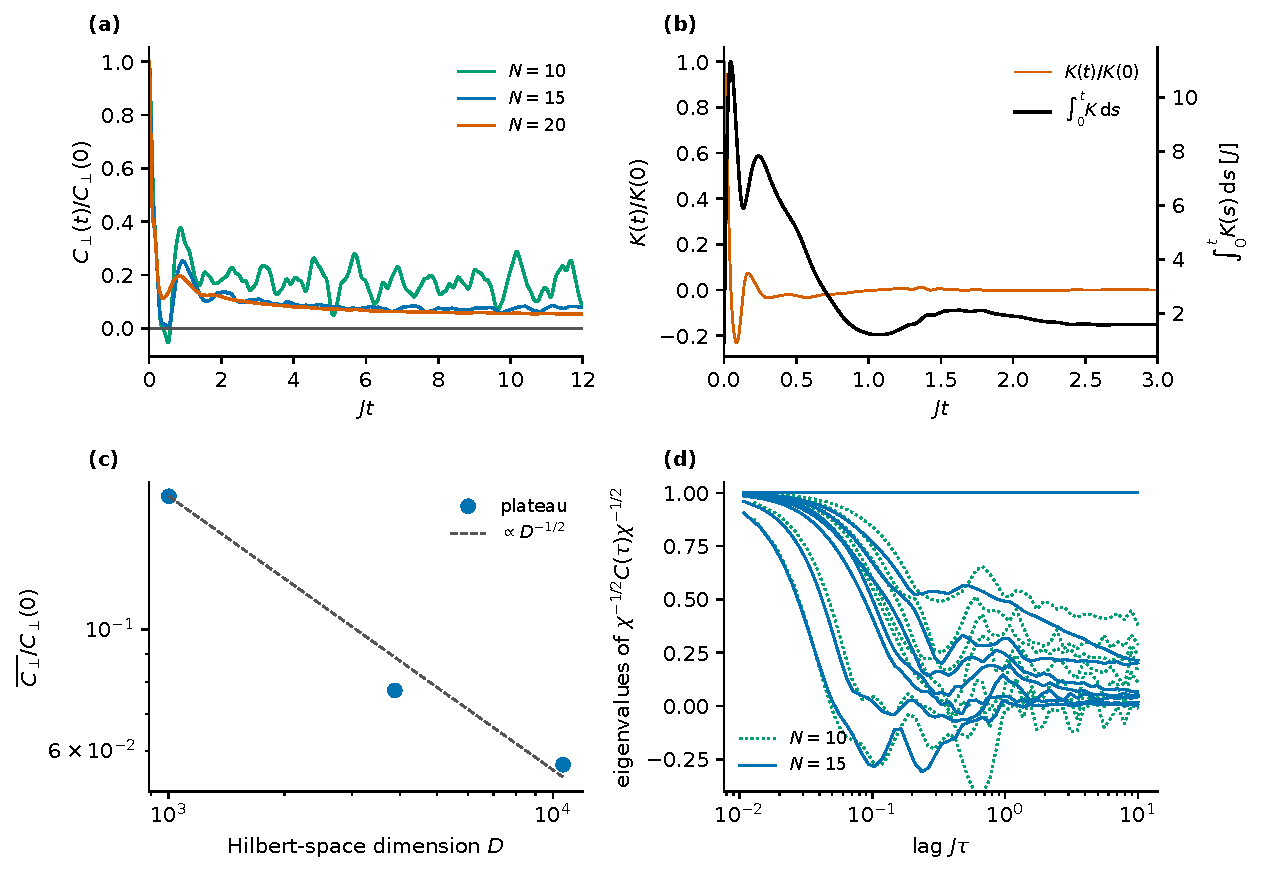
\includegraphics[width=0.92\textwidth]{lenk_mz.pdf}
  \caption{Mori--Zwanzig analysis in equilibrium (canonical state at the energy of the Fock state $ n_1 = N $). (a) Kubo relaxation function of the component of $ \hat n_{\mathrm{sys}} = \hat n_3 + \hat n_4 + \hat n_5 $ orthogonal to $ \hat H $. (b) Its memory kernel (left axis) and the running integral of the kernel (right axis), $ N = 20 $. (c) Infinite-time plateau of (a) versus Hilbert-space dimension; dashed: $ D^{-1/2} $. (d) Relaxation spectrum, Eq.~\eqref{eq:propagator}, of eight candidate slow variables; the eigenvalue $ 1 $ belongs to the energy.}
  \label{fig:lenk-mz}
\end{figure}

\subsection{Relaxation of the observed subsystem after a quench}
\label{sec:lenk-quench}

Figure~\ref{fig:lenk-quench} shows the dynamics from the Fock state $ n_1 = N = 20 $, the non-equilibrium initial state of Ref.~\cite{Lenk2025}.
Two stages are visible.
\begin{itemize}[leftmargin=1.5em]
\item Fast stage, $ Jt \lesssim 0.1 $. $ \langle\hat n_1\rangle $ drops from $ 20 $ to $ 11 $, and the Shannon entropy of the Fock-diagonal part of the reduced density matrix of S nearly reaches its final value. The time scale is the inverse energy width of the initial state, $ 1/\sigma_E = 0.023/J $ ($ \sigma_E = 44 $): the Fock state decays into the eigenstates it overlaps with, and the coherences between the Fock configurations it feeds dephase.
\item Slow stage, $ 0.3 \lesssim Jt \lesssim 5 $. The occupations approach their stationary values with damped oscillations, and the von Neumann entropy of S rises to its stationary value. The mean deviation of this entropy from its final value decreases from $ 0.44 $ ($ 0.6 < Jt < 1.2 $) to $ 0.16 $, $ 0.07 $ and $ 0.03 $ in the successive doubled windows, i.e.\ with an effective time constant of $ 1/J $ to $ 2/J $ that grows with time. A single exponential does not describe the stage.
\end{itemize}
The two stages are not the relaxation of two modes, since the relaxation spectrum has no gap; they are the initial dephasing, on the scale $ 1/\sigma_E $, followed by the non-Markovian relaxation of Sec.~\ref{sec:lenk-mz}.

The stationary values are close to thermal ones.
The long-time occupations, $ (7.53, 4.69, 3.43, 2.48, 1.88) $, agree with the canonical values at the same mean energy, $ (7.53, 4.90, 3.36, 2.41, 1.80) $, within $ 4\% $.
At $ N = 25 $ the agreement is $ 9\% $ for $ n_1 $ and better than $ 5\% $ for the other levels: $ (6.61, 6.05, 4.93, 4.04, 3.36) $ versus $ (7.28, 5.80, 4.72, 3.91, 3.29) $.
The deviations do not decrease monotonically with $ N $ in this range.
The deviations are not caused by the energy distribution of the initial state: averaging the smooth energy dependence of the eigenstate expectation values $ \langle a | \hat n_i | a \rangle $ over that distribution reproduces the canonical values to $ 1 $--$ 3\% $ (checked for $ N = 10, 15 $).
They come from the fluctuations of $ \langle a | \hat n_i | a \rangle $ between neighbouring eigenstates, which are correlated with the overlaps $ |\langle a | \psi(0) \rangle|^2 $ of the initial Fock state: a finite-size memory of the initial condition, of the same origin as the plateau of Fig.~\ref{fig:lenk-mz}(c).

For the entropy, the appropriate reference is not the thermal entropy of S.
The global state is pure, so the entropy of S equals that of R, and R contains at most $ N - n_{\mathrm{sys}} + 1 $ states for each value of $ n_{\mathrm{sys}} $.
The Schmidt rank is therefore at most $ \sum_{n_{\mathrm{sys}}} \min(d_S, d_R) $, with $ d_S $ and $ d_R $ the dimensions of the two factors in each block, which bounds the entropy by $ \ln 171 = 5.14 $ for $ N = 20 $ and $ \ln 266 = 5.58 $ for $ N = 25 $.
Neither part is small compared with the other, so the entropy of a pure state stays below the thermal entropy of either part.
The reference is the entropy of S in a canonical-typical pure state, $ |\psi\rangle = \sum_a \sqrt{p_a} \, e^{\ii\varphi_a} |a\rangle $ with canonical weights $ p_a $ and random phases $ \varphi_a $: $ 4.786 \pm 0.010 $ for $ N = 20 $.
The long-time value after the quench is $ 4.585 \pm 0.010 $, $ 4\% $ lower.
The late-time state differs from a canonical-typical state only in its weights $ |\langle a | \psi(0) \rangle|^2 $, so the difference is due to these weights. They differ from the canonical ones both in their energy distribution, which is half as wide [Fig.~\ref{fig:lenk-quench}(c)], and in their eigenstate-to-eigenstate structure.
At $ N = 25 $ the long-time entropy is $ 5.145 \pm 0.006 $, which reproduces $ \bar S_\infty = 5.15 $ of Ref.~\cite{Lenk2025}, while the canonical-typical value is $ 5.354 \pm 0.002 $, again $ 4\% $ higher.
The observed subsystem thus thermalizes, in the sense that its few-body observables and its entanglement entropy reach the values of a thermal pure state of the whole, up to deviations of a few per cent (at most $ 9\% $ for the occupations at $ N = 25 $) that reflect a finite-size memory of the initial state.

\begin{figure}[t]
  \centering
  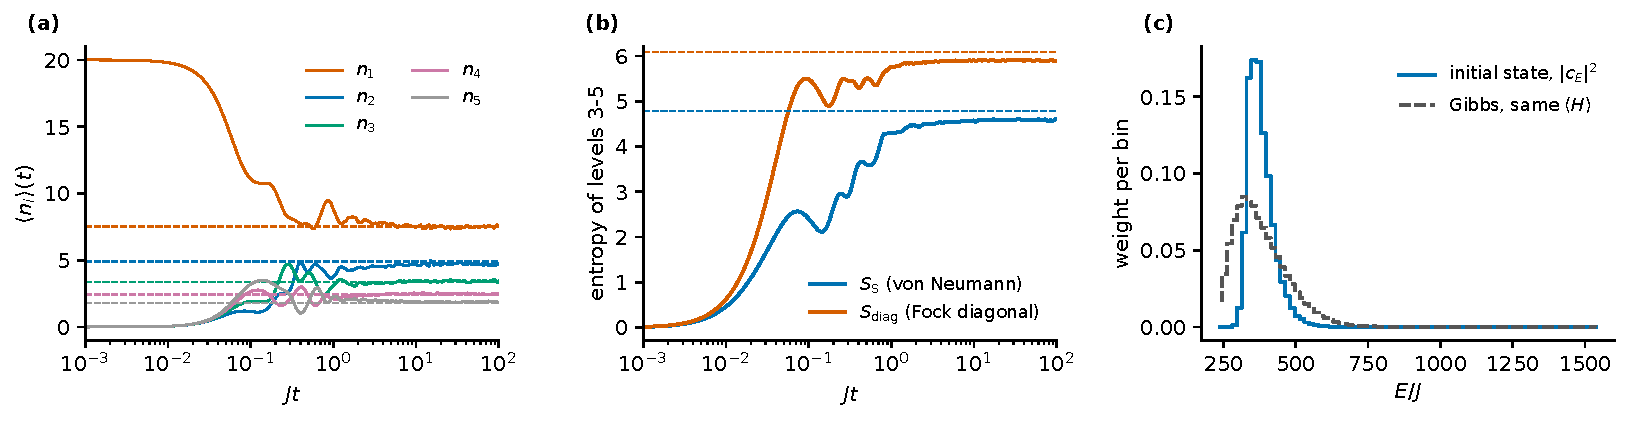
\includegraphics[width=\textwidth]{lenk_quench.pdf}
  \caption{Quench from the Fock state $ n_1 = N = 20 $. (a) Level occupations; dashed: canonical values at the same mean energy. (b) Von Neumann entropy of the reduced state of levels 3--5, and Shannon entropy of its Fock-diagonal part; dashed: values for canonical-typical pure states. (c) Energy distribution of the initial state, a constant of motion, compared with the canonical distribution with the same mean energy.}
  \label{fig:lenk-quench}
\end{figure}

\subsection{The whole does not thermalize}

The whole remains far from equilibrium, in three exactly verifiable ways.
First, its state is pure at all times, with zero entropy, while every Gibbs state has an extensive one.
Second, the energy distribution $ p_E = |\langle E | \psi(0) \rangle|^2 $ is a constant of motion; for the Fock initial state at $ N = 20 $ it has width $ \sigma_E = 44 $, compared with $ 90 $ for the canonical state [Fig.~\ref{fig:lenk-quench}(c)], and it keeps this form forever.
Third, the trace distance to any Gibbs state is constant, by Eq.~\eqref{eq:invariants}.
What thermalizes is the reduced description of the observed levels, whose environment, the remaining degrees of freedom of the same closed system, acts as an internal bath.

\subsection{Critique of Lenk et al.}
\label{sec:lenk-critique}

The numerical findings \ref{r:entropy} and \ref{r:nsys} and the near-thermal occupations are reproduced here; at $ N = 25 $ the stationary entropy agrees with $ \bar S_\infty = 5.15 $ to three digits.
The authors' central idea is also supported: the unobserved part of a closed, non-integrable system acts as a reservoir for the observed part, and the subsystem, not the whole, approaches thermal behaviour.
The interpretation, however, needs the following corrections.
\begin{enumerate}[label=(\alph*), leftmargin=2.2em]
\item Measurement plays no dynamical role. The partition into S and R is a choice of relevant variables, i.e.\ of the projector $ \PP $, and the reduced dynamics is the same whether or not a measurement is made. ``Measurement-induced bath generation'' is therefore not a separate mechanism: it is the relaxation of a subsystem inside a closed chaotic system. What makes R act as a bath is the dephasing of the memory kernel over $ \propto D $ incommensurate frequencies (Sec.~\ref{sec:mz-method}), which requires non-integrability, as the authors state; the partition alone does not. For $ U = U' = 0 $ the Hamiltonian is quadratic, its single-particle eigenmode occupations are conserved, and the same partition would produce entanglement but relaxation to a GGE.
\item The ``bath'' is not the larger part. R holds most of the particles, but in each block of fixed $ n_{\mathrm{sys}} $ it has at most $ N - n_{\mathrm{sys}} + 1 \le 26 $ states, fewer than S for most blocks. The entanglement entropy is bounded by $ \ln 266 = 5.58 $ at $ N = 25 $ and saturates at the value of a thermal pure state, not at a thermal entropy of S. The claim that the maximum of the entanglement entropy ``represents a thermal state'' is tested in Ref.~\cite{Lenk2025} only indirectly, through \ref{r:spectra} and \ref{r:corr}; the direct test is the comparison with a canonical-typical pure state made above.
\item The two time constants are not two relaxation modes. The relaxation spectrum has no gap [Fig.~\ref{fig:lenk-mz}(d)], and the memory kernel of $ n_{\mathrm{sys}} $ gives no Markov rate. The fast constants of \ref{r:entropy} and \ref{r:nsys} differ by a factor of six ($ 0.26/J $ and $ 0.041/J $); the faster one is of the order of the inverse energy width of the initial state, $ 1/\sigma_E = 0.017/J $ at $ N = 25 $ ($ \sigma_E = 60 $), the time on which the Fock state decays into eigenstates. The bi-exponential form describes the data in the fit window but carries no further physical content.
\item The narrow state is static for a different reason than stated in \ref{r:narrow}. Its $ 74 $ eigenstates span $ 1.7\,J $, so its dynamics is not restricted to a single frequency. It is static because an equal-weight superposition of many eigenstates in a narrow window is already a typical state, whose reduced state is thermal at $ t = 0 $ (canonical typicality~\cite{Goldstein2006,Popescu2006}); accordingly its initial entanglement entropy is already large.
\item Broad energy distributions and correlations between levels are within the scope of the ETH. For any initial state, stationary expectation values are diagonal-ensemble averages, $ \sum_a |\langle a|\psi(0)\rangle|^2 \langle a|\hat O|a\rangle $; the ETH makes them thermal when $ \langle a|\hat O|a\rangle $ varies smoothly on the scale of the energy width, here $ \sigma_E/E \approx 0.1 $. With five levels, the products $ \hat n_i \hat n_j $ are few-body operators to which the ETH applies. The residual deviations found above are finite-size fluctuations of exactly the kind the ETH describes. The ETH indeed does not predict rates, since it leaves the function $ f_O $ of Eq.~\eqref{eq:eth} unspecified, but neither does the bath-generation picture: the time constants of \ref{r:entropy}--\ref{r:nsys} and the temperature of \ref{r:spectra} are numerical results, not predictions. The Mori--Zwanzig kernel is the framework in which rates can be computed.
\item The temperature fit has one free parameter too few. Setting $ \mu = 0 $ is justified in Ref.~\cite{Lenk2025} by the particle number of S not being fixed; but a subsystem exchanging particles with R has the chemical potential of R, which is not zero in general, while the total $ N $ is fixed. At $ T/J \approx 200 $, well above most peak energies $ E_i $, the Bose function is close to $ T/E_i - \frac12 $, and $ \sum_i n_i = N $ then fixes $ T \simeq (N + M/2) / \sum_i E_i^{-1} $: the fitted temperature is largely determined by the particle number and the peak positions. The fitted value nevertheless lies within $ 5\% $ of the canonical temperature of the whole at the quench energy, $ T/J = 207 $ at $ N = 25 $: the single-particle spectra are consistent with the many-body temperature, but the fit with $ \mu $ fixed tests the high-temperature shape $ n_i \propto 1/E_i $ rather than determining $ T $ and $ \mu $ independently. The extraction formula printed in Ref.~\cite{Lenk2025}, $ n_{\mathrm B} = \ii \bar G^K_i/\bar A_i - \frac12 $, is inconsistent with their fluctuation--dissipation relation $ G^K = -\ii A (2 n_{\mathrm B} + 1) $, which gives $ n_{\mathrm B} = (\ii G^K/A - 1)/2 $; this is presumably a misprint.
\item The role of the Hilbert-space dimension is confirmed, with a caveat. Finite-size memory scales as $ D^{-1/2} $ [Fig.~\ref{fig:lenk-mz}(c)], supporting the statement that $ D $, not $ N $, controls the approach to the thermodynamic limit. At fixed $ M = 5 $, however, $ N \to \infty $ is the semiclassical limit, with effective Planck constant $ \propto 1/N $, of a system of five coupled nonlinear modes, whose ergodicity is not guaranteed by the growth of $ D $.
\end{enumerate}

%======================================================================
\section{Conclusions and Outlook}
\label{sec:conclusion}

Table~\ref{tab:summary} collects the four cases.
In all of them the whole does not thermalize, as required by Eq.~\eqref{eq:invariants}.
A reduced description reaches a steady state when its memory kernel decays.
In a closed system this happens by dephasing, not by loss of information. It requires a bath, external or internal, large enough that its frequencies are dense on the time scale of observation, and free of additional conservation laws that would keep part of the kernel from decaying.
The steady state is a Gibbs state at a given temperature when the bath obeys detailed balance at that temperature.
When the reduced variables are, in addition, weakly coupled to the bath, i.e.\ slow in the sense of Eq.~\eqref{eq:markov-condition}, the approach is Markovian and follows from the bath's two-point function alone.
An external bath that is large, weakly coupled and thermal supplies all of this (Secs.~\ref{sec:bath}, \ref{sec:quantum}).
Inside a closed system, the remaining degrees of freedom can act as the bath (Sec.~\ref{sec:mz} and Appendix~\ref{app:fput}).
In the Bose gas of Lenk \textit{et al.}\ they do: the observed occupations reach values within a few per cent of thermal ones, with a finite-size memory that scales as $ D^{-1/2} $ in equilibrium. But the relaxation spectrum has no gap, so the only slow variable is the energy, and the approach is non-Markovian.

More generally, slow and fast are the two ends of a hierarchy of relaxation rates.
Which variables form the system and which the bath is fixed by the time scale of observation: faster variables have relaxed and act as the bath, slower ones are frozen and act as constants of motion, and the state reached is the constrained equilibrium~\eqref{eq:constrained}, with a multiplier, and possibly a temperature, for each frozen variable.
The line between system and bath is well defined only where the rates have a gap; in the Bose gas they have none.

\begin{table}[h]
\centering
\small
\renewcommand{\arraystretch}{1.25}
\setlength{\tabcolsep}{4pt}
\begin{tabular}{p{0.18\textwidth} p{0.19\textwidth} p{0.22\textwidth} p{0.13\textwidth} p{0.2\textwidth}}
\hline
System & Method & Mechanism & Whole & Reduced description \\
\hline
Harmonic chain (Sec.~\ref{sec:chain}) & normal modes, exact & none: $ N $ conserved mode energies & not thermal & not thermal (GGE) \\
$ \beta $-FPUT chain (Appendix~\ref{app:fput}) & symplectic integration & mode coupling by anharmonicity & not thermal & mode energies equipartition \\
Harmonic system + large bath (Sec.~\ref{sec:bath}) & exact elimination, second-order averaging, exact numerics & golden-rule exchange with a thermal continuum & not thermal & Gibbs at bath $ T $ \\
Quantum system + bosonic bath (Sec.~\ref{sec:quantum}) & Wick identity, Born--Markov--secular (Davies) & golden-rule rates with KMS detailed balance & not thermal & Gibbs at KMS $ \beta $ \\
Isolated Bose gas (Sec.~\ref{sec:mz}) & Mori--Zwanzig, exact diagonalization & internal bath, strongly coupled, non-Markovian & pure; $ p_E $ conserved & within a few \% of thermal; residual memory ($ \propto D^{-1/2} $ in equilibrium) \\
\hline
\end{tabular}
\caption{Summary: whether the whole and a reduced description thermalize, and why.}
\label{tab:summary}
\end{table}

The following calculations and experiments would extend these results.
\begin{itemize}[leftmargin=1.5em]
\item Determine the conditions under which an internal bath is weakly coupled. Candidates are few observed levels tunnel-coupled to a large, dense set of unobserved levels, for which $ K(0)\tau_c^2 $ can be tuned, and larger $ M $ at fixed filling. Krylov or dynamical-typicality methods reach Hilbert-space dimensions of $ 10^8 $ and would show whether a Markovian window opens with system size.
\item Compute the Nakajima--Zwanzig kernel for the Fock populations of Eq.~\eqref{eq:lenk-H}. It would connect the fast decay of the initial state (width $ \sigma_E $) and the slow redistribution to explicit rates, and identify the non-Markovian corrections responsible for the revivals.
\item Test the thermality of reduced states by the generalized fluctuation--dissipation relation~\eqref{eq:beta-eff}, i.e.\ by measuring noise and response of the same observable, in systems with controllable coupling to a bath (superconducting circuits, trapped-ion phonon modes, nanomechanical resonators), from weak coupling, where $ \beta_{\mathrm{eff}} $ should be constant, to strong coupling, where the Hamiltonian of mean force takes over.
\item In ultracold gases in multi-level traps or coupled condensates~\cite{Posazhennikova2016}, compare the relaxation of level occupations with and without an integrability-breaking perturbation~\cite{Kinoshita2006,Langen2015}, and measure the finite-size residual fluctuations predicted to scale as $ D^{-1/2} $.
\item Measure the temperature dependence of Debye--Waller factors or interferometric visibilities together with the lattice entropy, to test the relation between single-probe decoherence and bulk thermodynamics (Sec.~\ref{sec:debye}).
\end{itemize}

%======================================================================
\appendix

\section{Integrable and Non-Integrable Dynamics}
\label{app:integrability}

Whether a system has conserved quantities beyond the energy (Sec.~\ref{sec:defs}) is the distinction between integrable and non-integrable systems.

\paragraph{Classical systems.}
A Hamiltonian system with $ f $ degrees of freedom is (Liouville) integrable if it has $ f $ independent constants of motion $ I_1, \dots, I_f $ in involution, $ \{ I_k , I_l \} = 0 $.
Each trajectory then lies on an $ f $-dimensional torus labelled by the values of the $ I_k $. In the action--angle variables of that torus the actions are constant and the angles advance uniformly, so the motion is quasi-periodic.
A trajectory explores only its torus, not the energy shell.
A system with fewer than $ f $ such constants is non-integrable.
Non-integrability is the generic case: an arbitrary interaction destroys the extra constants of motion, and parts of the energy shell become chaotic, with nearby trajectories separating exponentially in time.
A weak perturbation of an integrable system is special: by the Kolmogorov--Arnold--Moser (KAM) theorem, most tori then survive in deformed form, and chaos is confined to thin layers between them~\cite{Berman2005}.

\paragraph{Quantum systems.}
Counting conserved operators does not work in quantum mechanics, because every Hamiltonian has as many commuting constants of motion as its Hilbert-space dimension: the projectors $ |a\rangle\langle a| $ onto its eigenstates.
The accepted working definition~\cite{Caux2011} counts only conserved quantities with physical structure, i.e.\ sums of few-body (or local) operators.
A many-body system is integrable if it has a number of independent such conserved quantities that grows with the number of degrees of freedom; it is non-integrable if only a few exist, typically the energy, the particle number and the momentum.
The standard example of an integrable system is a quadratic Hamiltonian, whose single-particle eigenmode occupations are all conserved; interacting models solvable by the Bethe ansatz are others.
An operational test is the statistics of the energy levels.
Levels of integrable systems are uncorrelated (Poisson statistics), because the many conserved quantities split the spectrum into independent sectors.
Levels of non-integrable systems repel each other and follow random-matrix (Wigner--Dyson) statistics~\cite{BerryTabor1977,Bohigas1984}.
A convenient measure is the mean ratio $ \langle r \rangle $ of consecutive level spacings~\cite{Oganesyan2007,Atas2013}: $ \langle r\rangle \simeq 0.386 $ for Poisson statistics and $ 0.531 $ for the Gaussian orthogonal ensemble of real symmetric random matrices.
Non-integrability is the quantum counterpart of chaos, and it is the condition under which few-body observables of a closed system are expected to thermalize~\cite{DAlessio2016}.

\section{The Eigenstate Thermalization Hypothesis}
\label{app:eth}

\paragraph{The question.}
A closed quantum system prepared in a pure state $ |\psi(0)\rangle = \sum_a c_a |a\rangle $, with energy eigenstates $ |a\rangle $, evolves as
\begin{equation}
  \langle \hat O \rangle(t) = \sum_{a,b} c_a^* c_b \, e^{\ii(E_a - E_b)t} \, O_{ab} ,
  \qquad
  O_{ab} = \langle a | \hat O | b \rangle .
  \label{eq:eth-evolution}
\end{equation}
For non-degenerate energies the off-diagonal terms dephase, and the long-time average is the diagonal-ensemble average $ \bar O = \sum_a |c_a|^2 O_{aa} $.
It depends on all $ D $ weights $ |c_a|^2 $, which are constants of motion.
Thermalization requires instead that $ \bar O $ depend only on the energy.
The eigenstate thermalization hypothesis (ETH) explains how, through a property of the matrix elements $ O_{ab} $.
Its precursor is von Neumann's quantum ergodic theorem~\cite{vonNeumann1929,Goldstein2010}.
It was formulated by Deutsch~\cite{Deutsch1991}, for an integrable Hamiltonian perturbed by a random matrix, and by Srednicki~\cite{Srednicki1994}, for chaotic systems whose eigenfunctions behave as random superpositions of plane waves (Berry's conjecture~\cite{Berry1977}). Srednicki extended it to off-diagonal elements~\cite{Srednicki1999}. It was verified numerically for interacting lattice bosons by Rigol, Dunjko and Olshanii~\cite{Rigol2008}. Comprehensive reviews are Refs.~\cite{DAlessio2016,Deutsch2018}.

\paragraph{Premises.}
\begin{enumerate}[label=(P\arabic*), leftmargin=3.0em]
\item The Hamiltonian is non-integrable (Appendix~\ref{app:integrability}), with Wigner--Dyson level statistics.
\item The observable is few-body or local. The hypothesis is not meant for arbitrary operators, such as the projectors $ |a\rangle\langle a| $, which are conserved.
\item The eigenstates lie in the bulk of the spectrum, where the density of states $ e^{S(E)} $ is large. $ S(E) $ is the thermodynamic entropy of the whole at energy $ E $.
\item The statements are asymptotic in system size; corrections are controlled by $ e^{-S/2} $.
\end{enumerate}

\paragraph{Statement.}
In the form given by Srednicki~\cite{Srednicki1999},
\begin{equation}
  O_{ab} = O(\bar E) \, \delta_{ab} + e^{-S(\bar E)/2} \, f_O(\bar E, \omega) \, R_{ab} ,
  \qquad
  \bar E = \tfrac12 (E_a + E_b) , \quad \omega = E_b - E_a .
  \label{eq:eth}
\end{equation}
Here $ O(E) $ and $ f_O(E,\omega) $ are smooth functions of their arguments, and $ R_{ab} $ are pseudo-random numbers with zero mean and unit variance.
$ O(E) $ equals the microcanonical average of $ \hat O $ at energy $ E $.
Hermiticity of $ \hat O $ requires $ |f_O(E,-\omega)| = |f_O(E,\omega)| $.
The diagonal elements are thus a smooth function of energy, up to fluctuations of relative size $ e^{-S/2} $ between neighbouring eigenstates.
The off-diagonal elements are exponentially small, with a smooth frequency profile $ f_O $.
The weak form of the hypothesis requires this for most eigenstates; the strong form requires it for all eigenstates in the bulk of the spectrum~\cite{Biroli2010,Kim2014}.

\paragraph{Consequences.}
\begin{enumerate}[label=(E\arabic*), leftmargin=3.0em]
\item Stationary values. For an initial state with mean energy $ E $ and energy width $ \delta E $, Eq.~\eqref{eq:eth} gives $ \bar O = O(E) + \tfrac12 O''(E)\,\delta E^2 + O(e^{-S/2}) $. For local Hamiltonians $ \delta E $ grows only as the square root of the system size, while $ O(E) $ varies on extensive energy scales, so $ \bar O $ approaches the microcanonical value. The initial state is forgotten except for its energy, for broad as well as narrow energy distributions in this sense. In an integrable system $ O_{aa} $ depends on all conserved quantities, not on the energy alone, and $ \bar O $ is a GGE average.
\item Small temporal fluctuations. For non-degenerate energy gaps, the time-averaged squared deviation from $ \bar O $ is
\begin{equation*}
  \overline{\big( \langle\hat O\rangle(t) - \bar O \big)^2}
  = \sum_{a \neq b} |c_a|^2 |c_b|^2 |O_{ab}|^2
  \le \max_{a\neq b} |O_{ab}|^2 \sum_a |c_a|^4 ,
\end{equation*}
with $ \max |O_{ab}|^2 \propto e^{-S} $ by Eq.~\eqref{eq:eth}. Once dephased, the expectation value stays close to $ \bar O $ for almost all times~\cite{Reimann2008}.
\item Thermal eigenstates. A single eigenstate reproduces the thermal values of all few-body observables. The reduced density matrix of a subsystem that is small compared with the rest is thermal in each eigenstate~\cite{Garrison2018}. Thermalization is thus encoded in the eigenstates; the dynamics only dephases the initial superposition, the mechanism of Sec.~\ref{sec:mz-method}.
\item Detailed balance within an eigenstate. In the eigenstate $ |a\rangle $, the correlation functions of Eq.~\eqref{eq:bath-corr} become $ C^>(\omega) = 2\pi \sum_b |O_{ab}|^2 \delta(\omega - E_b + E_a) = 2\pi |f_O(E_a + \omega/2, \omega)|^2 \, e^{S(E_a + \omega) - S(E_a + \omega/2)} $, and similarly for $ C^< $ with $ \omega \to -\omega $. Expanding the entropies to first order in $ \omega $ gives $ C^>(\omega)/C^<(\omega) = e^{\beta\omega} $ with $ \beta = \partial S/\partial E $. Each eigenstate thus satisfies the KMS condition at the microcanonical temperature, and the fluctuation--dissipation theorem holds for few-body observables of a closed system~\cite{DAlessio2016}. The temperature enters through the density of states of the whole.
\item Finite-size corrections. The eigenstate-to-eigenstate fluctuations of $ O_{aa} $, of order $ e^{-S/2} $, are the finite-size memory of the initial state. Their scaling has been verified numerically in lattice models~\cite{Beugeling2014,Kim2014}. In the Bose gas of Sec.~\ref{sec:mz}, $ e^{S} $ is proportional to $ D $, and the $ D^{-1/2} $ plateau of Fig.~\ref{fig:lenk-mz}(c) is this prediction.
\end{enumerate}

\paragraph{Limits.}
The ETH is a hypothesis, supported by extensive numerical evidence and proved only for random-matrix models.
It fails for integrable systems, where the stationary state is a GGE; for many-body localized systems, whose eigenstates are not thermal~\cite{Nandkishore2015}; and for rare non-thermal eigenstates (quantum many-body scars) in otherwise chaotic systems~\cite{Turner2018}.
It leaves the function $ f_O(E,\omega) $ unspecified, and with it the relaxation times: the ETH predicts where a system relaxes to, not how fast.
Canonical typicality~\cite{Goldstein2006,Popescu2006} is a complementary, kinematic statement: most pure states in an energy shell have thermal reduced states. The ETH states that every eigenstate is such a state, which guarantees relaxation from any initial state with a sufficiently narrow energy distribution, not only from typical ones.

\section{Anharmonic Chain: The FPUT Problem}
\label{app:fput}

The chain of Sec.~\ref{sec:chain-numerics} is the one studied numerically by Fermi, Pasta, Ulam and Tsingou (FPUT)~\cite{FPU1955}, who expected an anharmonic coupling of the modes to produce equipartition.
Adding a quartic term to the spring potential, $ V(r) = \kappa r^2/2 + \beta r^4/4 $ with $ r = x_{j+1} - x_j $, couples the normal modes.
This is the $ \beta $-FPUT chain~\cite{FPU1955,Berman2005}, named after the coefficient $ \beta $ of the quartic term (a cubic term, with coefficient $ \alpha $, defines the $ \alpha $-FPUT chain).
The chain remains closed, conserves energy, and still obeys Eq.~\eqref{eq:invariants}, but it is no longer integrable.
With $ \beta = \kappa/a^2 $ and the same initial conditions as in Fig.~\ref{fig:chain}, $ n_{\mathrm{eff}} $ reaches the equipartition value for $ \omega_0 t \gtrsim 3\times 10^3 $, $ c_1 $ decays to zero, and the long-time mode spectrum is flat (Fig.~\ref{fig:fput}).
The distribution of mode energies, a reduced description, has thermalized: each mode exchanges energy with all others, which act as its bath.
This is the classical counterpart of the internal bath analyzed in Sec.~\ref{sec:mz}.
The obstacle to thermalization in Sec.~\ref{sec:chain} is therefore integrability, not the closedness of the chain.
Near integrability the approach can be very slow, since by the KAM theorem (Appendix~\ref{app:integrability}) many invariant tori survive a weak nonlinearity~\cite{Berman2005}.

\begin{figure}[t]
  \centering
  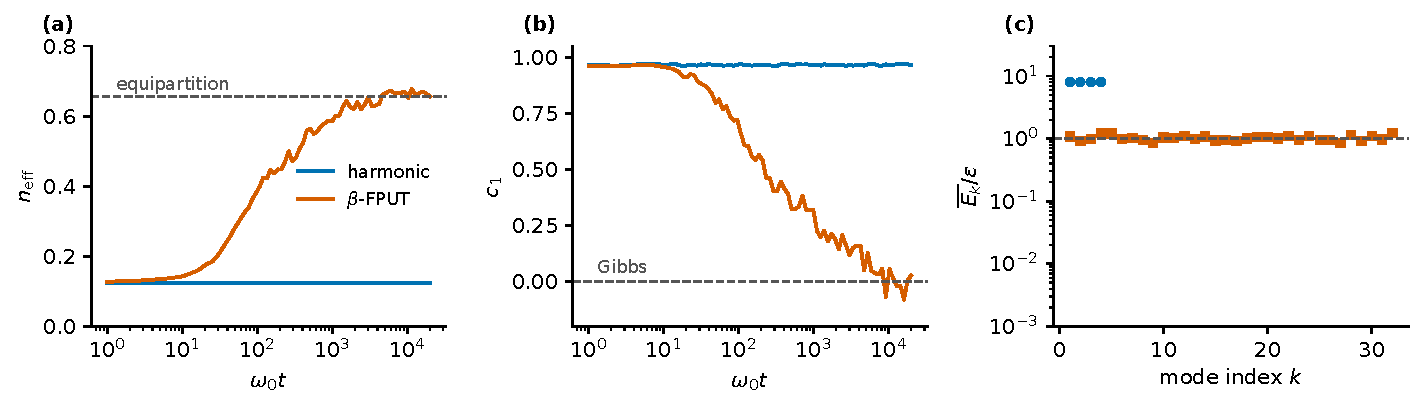
\includegraphics[width=\textwidth]{fput.pdf}
  \caption{Harmonic (blue) versus $ \beta $-FPUT (red, $ \beta = \kappa/a^2 $) chain, same initial conditions as Fig.~\ref{fig:chain}. (a) Effective fraction of excited modes; dashed: equipartition value. (b) Nearest-neighbour momentum correlation; dashed: Gibbs value. (c) Mode energies averaged over $ 10^4 < \omega_0 t < 2\times 10^4 $ (logarithmic scale); harmonic modes $ k > 4 $ carry no energy and lie below the axis.}
  \label{fig:fput}
\end{figure}

\section{Numerical Methods}
\label{app:numerics}

The Python scripts in \texttt{code/} generate all figures (\texttt{make figs}).

\paragraph{Harmonic and FPUT chains (Figs.~\ref{fig:chain}, \ref{fig:fput}).}
Units $ m = \kappa = a = 1 $. The equations of motion are integrated with the fourth-order symplectic scheme of Yoshida~\cite{Yoshida1990}, $ \delta t = 0.05 $, up to $ \omega_0 t = 2\times 10^4 $. A symplectic scheme preserves phase-space volume and keeps the energy error bounded; the relative energy error is below $ 10^{-5} $. Mode energies are projections onto the sine modes of Eq.~\eqref{eq:chain-modes}.

\paragraph{System coupled to a bath (Fig.~\ref{fig:bath}).}
Units $ \omega_0 = \kB T = 1 $. The bath frequencies are $ \omega_k = (k - \tfrac12)\,\delta\omega $ with $ \delta\omega = \omega_c/N_B $, and $ c_k^2 = (2/\pi)\,\eta\,\omega_k^2\,\delta\omega $ reproduces the Ohmic density~\eqref{eq:Jclass}. The $ (N_B + 2) \times (N_B + 2) $ stiffness matrix of Eqs.~\eqref{eq:HS}--\eqref{eq:HB} is diagonalized, and the exact solution~\eqref{eq:chain-solution} is evaluated for 4000 realizations: random phases of the system modes, and bath coordinates drawn from the Gibbs state around the displaced equilibrium $ q_k = c_k x_1(0)/\omega_k^2 $.

\paragraph{Bose gas (Figs.~\ref{fig:lenk-mz}, \ref{fig:lenk-quench}).}
The Hamiltonian is built in the Fock basis from Eq.~\eqref{eq:lenk-K}, verified against the term-by-term definition~\eqref{eq:lenk-H} for small $ N $, and diagonalized with LAPACK (80~s for $ D = 10626 $). The Kubo relaxation function is
\begin{equation}
  C(t) = \sum_{a,b} \frac{p_a - p_b}{\beta (E_b - E_a)} \, |A_{ab}|^2 \cos\big[(E_b - E_a) t\big] - \langle A \rangle^2 ,
  \label{eq:kubo-spectral}
\end{equation}
with $ p_a \propto e^{-\beta E_a} $, $ A_{ab} = \langle a | \hat n_{\mathrm{sys}} | b \rangle $, and the factor replaced by $ p_a $ for $ a = b $. The weights are binned on a frequency grid of spacing $ 0.005\,J $ and Fourier transformed. The Mazur term $ \sprod{A}{H}^2/\sprod{H}{H} $ is subtracted, and Eq.~\eqref{eq:volterra} is solved with the trapezoidal rule on the resulting time grid ($ \delta t \approx 2\times 10^{-3}/J $). The quench is propagated exactly in the eigenbasis at 250 logarithmically spaced times. The relaxation spectrum uses the same binned Fourier transform for all pairs of the eight candidate variables ($ N = 10, 15 $). The $ N = 25 $ quench observables ($ D = 23\,751 $, diagonalization about 15~min) are computed by \texttt{code/lenk\_check.py}; the late-time entropy is averaged over 41 times in $ 20 \le Jt \le 100 $. Reduced density matrices of levels 3--5 are assembled block by block in $ n_{\mathrm{sys}} $. The canonical-typical reference is averaged over 8 sets of random phases.

%======================================================================
\begin{thebibliography}{99}
\small

\bibitem{Lenk2025}
M.~Lenk, S.~Biswas, A.~Posazhennikova, and J.~Kroha, Entropy \textbf{27}, 636 (2025), \href{https://doi.org/10.3390/e27060636}{doi:10.3390/e27060636}.

\bibitem{Rigol2007}
M.~Rigol, V.~Dunjko, V.~Yurovsky, and M.~Olshanii, Phys.\ Rev.\ Lett.\ \textbf{98}, 050405 (2007).

\bibitem{ThorntonMarion2004}
S.~T.~Thornton and J.~B.~Marion, \textit{Classical Dynamics of Particles and Systems}, 5th ed.\ (Brooks/Cole, Belmont, 2004), Ch.~12.

\bibitem{FPU1955}
E.~Fermi, J.~Pasta, and S.~Ulam, Los Alamos Report LA-1940 (1955).

\bibitem{Berman2005}
G.~P.~Berman and F.~M.~Izrailev, Chaos \textbf{15}, 015104 (2005).

\bibitem{Caldeira1983}
A.~O.~Caldeira and A.~J.~Leggett, Physica A \textbf{121}, 587 (1983).

\bibitem{Zwanzig1973}
R.~Zwanzig, J.~Stat.\ Phys.\ \textbf{9}, 215 (1973).

\bibitem{Zwanzig2001}
R.~Zwanzig, \textit{Nonequilibrium Statistical Mechanics} (Oxford University Press, Oxford, 2001).

\bibitem{Risken1989}
H.~Risken, \textit{The Fokker--Planck Equation}, 2nd ed.\ (Springer, Berlin, 1989).

\bibitem{Jaynes1957}
E.~T.~Jaynes, Phys.\ Rev.\ \textbf{106}, 620 (1957).

\bibitem{Davies1974}
E.~B.~Davies, Commun.\ Math.\ Phys.\ \textbf{39}, 91 (1974).

\bibitem{Mahan2000}
G.~D.~Mahan, \textit{Many-Particle Physics}, 3rd ed.\ (Kluwer Academic/Plenum, New York, 2000).

\bibitem{Breuer2002}
H.-P.~Breuer and F.~Petruccione, \textit{The Theory of Open Quantum Systems} (Oxford University Press, Oxford, 2002).

\bibitem{Pauli1928}
W.~Pauli, in \textit{Probleme der modernen Physik}, edited by P.~Debye (Hirzel, Leipzig, 1928), p.~30.

\bibitem{vanHove1955}
L.~van Hove, Physica \textbf{21}, 517 (1955).

\bibitem{Spohn1978}
H.~Spohn, J.~Math.\ Phys.\ \textbf{19}, 1227 (1978).

\bibitem{Cugliandolo2011}
L.~F.~Cugliandolo, J.~Phys.\ A \textbf{44}, 483001 (2011).

\bibitem{Korringa1950}
J.~Korringa, Physica \textbf{16}, 601 (1950).

\bibitem{Anderson1967}
P.~W.~Anderson, Phys.\ Rev.\ Lett.\ \textbf{18}, 1049 (1967).

\bibitem{Nozieres1969}
P.~Nozi\`eres and C.~T.~De~Dominicis, Phys.\ Rev.\ \textbf{178}, 1097 (1969).

\bibitem{Goldstein2006}
S.~Goldstein, J.~L.~Lebowitz, R.~Tumulka, and N.~Zangh\`i, Phys.\ Rev.\ Lett.\ \textbf{96}, 050403 (2006).

\bibitem{Popescu2006}
S.~Popescu, A.~J.~Short, and A.~Winter, Nat.\ Phys.\ \textbf{2}, 754 (2006).

\bibitem{Deutsch1991}
J.~M.~Deutsch, Phys.\ Rev.\ A \textbf{43}, 2046 (1991).

\bibitem{Srednicki1994}
M.~Srednicki, Phys.\ Rev.\ E \textbf{50}, 888 (1994).

\bibitem{Rigol2008}
M.~Rigol, V.~Dunjko, and M.~Olshanii, Nature \textbf{452}, 854 (2008).

\bibitem{DAlessio2016}
L.~D'Alessio, Y.~Kafri, A.~Polkovnikov, and M.~Rigol, Adv.\ Phys.\ \textbf{65}, 239 (2016).

\bibitem{Nakajima1958}
S.~Nakajima, Prog.\ Theor.\ Phys.\ \textbf{20}, 948 (1958).

\bibitem{Zwanzig1960}
R.~Zwanzig, J.~Chem.\ Phys.\ \textbf{33}, 1338 (1960).

\bibitem{Zwanzig1961}
R.~Zwanzig, Phys.\ Rev.\ \textbf{124}, 983 (1961).

\bibitem{Mori1965}
H.~Mori, Prog.\ Theor.\ Phys.\ \textbf{33}, 423 (1965).

\bibitem{Forster1975}
D.~Forster, \textit{Hydrodynamic Fluctuations, Broken Symmetry, and Correlation Functions} (W.~A.~Benjamin, Reading, MA, 1975).

\bibitem{Grabert1982}
H.~Grabert, \textit{Projection Operator Techniques in Nonequilibrium Statistical Mechanics}, Springer Tracts in Modern Physics Vol.~95 (Springer, Berlin, 1982).

\bibitem{Kubo1957}
R.~Kubo, J.~Phys.\ Soc.\ Jpn.\ \textbf{12}, 570 (1957).

\bibitem{Kubo1966}
R.~Kubo, Rep.\ Prog.\ Phys.\ \textbf{29}, 255 (1966).

\bibitem{Mazur1969}
P.~Mazur, Physica \textbf{43}, 533 (1969).

\bibitem{Bogoliubov1946}
N.~N.~Bogoliubov, \textit{Problems of a Dynamical Theory in Statistical Physics} (1946), English translation in \textit{Studies in Statistical Mechanics}, Vol.~1, edited by J.~de~Boer and G.~E.~Uhlenbeck (North-Holland, Amsterdam, 1962).

\bibitem{WilsonKogut1974}
K.~G.~Wilson and J.~Kogut, Phys.\ Rep.\ \textbf{12}, 75 (1974).

\bibitem{Chen1996}
L.-Y.~Chen, N.~Goldenfeld, and Y.~Oono, Phys.\ Rev.\ E \textbf{54}, 376 (1996).

\bibitem{Feynman1972}
R.~P.~Feynman, \textit{Statistical Mechanics: A Set of Lectures} (Benjamin, Reading, 1972), Ch.~1.

\bibitem{Berges2004}
J.~Berges, Sz.~Bors\'anyi, and C.~Wetterich, Phys.\ Rev.\ Lett.\ \textbf{93}, 142002 (2004).

\bibitem{Kollar2011}
M.~Kollar, F.~A.~Wolf, and M.~Eckstein, Phys.\ Rev.\ B \textbf{84}, 054304 (2011).

\bibitem{Mori2018}
T.~Mori, T.~N.~Ikeda, E.~Kaminishi, and M.~Ueda, J.~Phys.\ B \textbf{51}, 112001 (2018).

\bibitem{Palmer1982}
R.~G.~Palmer, Adv.\ Phys.\ \textbf{31}, 669 (1982).

\bibitem{AbragamProctor1958}
A.~Abragam and W.~G.~Proctor, Phys.\ Rev.\ \textbf{109}, 1441 (1958).

\bibitem{Anisimov1974}
S.~I.~Anisimov, B.~L.~Kapeliovich, and T.~L.~Perel'man, Zh.\ Eksp.\ Teor.\ Fiz.\ \textbf{66}, 776 (1974) [Sov.\ Phys.\ JETP \textbf{39}, 375 (1974)].

\bibitem{Caux2011}
J.-S.~Caux and J.~Mossel, J.~Stat.\ Mech.\ (2011) P02023.

\bibitem{BerryTabor1977}
M.~V.~Berry and M.~Tabor, Proc.\ R.\ Soc.\ Lond.\ A \textbf{356}, 375 (1977).

\bibitem{Bohigas1984}
O.~Bohigas, M.~J.~Giannoni, and C.~Schmit, Phys.\ Rev.\ Lett.\ \textbf{52}, 1 (1984).

\bibitem{Oganesyan2007}
V.~Oganesyan and D.~A.~Huse, Phys.\ Rev.\ B \textbf{75}, 155111 (2007).

\bibitem{Atas2013}
Y.~Y.~Atas, E.~Bogomolny, O.~Giraud, and G.~Roux, Phys.\ Rev.\ Lett.\ \textbf{110}, 084101 (2013).

\bibitem{Posazhennikova2016}
A.~Posazhennikova, M.~Trujillo-Martinez, and J.~Kroha, Phys.\ Rev.\ Lett.\ \textbf{116}, 225304 (2016).

\bibitem{Kinoshita2006}
T.~Kinoshita, T.~Wenger, and D.~S.~Weiss, Nature \textbf{440}, 900 (2006).

\bibitem{Langen2015}
T.~Langen \textit{et al.}, Science \textbf{348}, 207 (2015).

\bibitem{Yoshida1990}
H.~Yoshida, Phys.\ Lett.\ A \textbf{150}, 262 (1990).

\bibitem{HHW1967}
R.~Haag, N.~M.~Hugenholtz, and M.~Winnink, Commun.\ Math.\ Phys.\ \textbf{5}, 215 (1967).

\bibitem{HKTP1974}
R.~Haag, D.~Kastler, and E.~B.~Trych-Pohlmeyer, Commun.\ Math.\ Phys.\ \textbf{38}, 173 (1974).

\bibitem{PuszWoronowicz1978}
W.~Pusz and S.~L.~Woronowicz, Commun.\ Math.\ Phys.\ \textbf{58}, 273 (1978).

\bibitem{Lenard1978}
A.~Lenard, J.~Stat.\ Phys.\ \textbf{19}, 575 (1978).

\bibitem{vonNeumann1929}
J.~von Neumann, Z.~Phys.\ \textbf{57}, 30 (1929); English translation in Eur.\ Phys.\ J.\ H \textbf{35}, 201 (2010).

\bibitem{Goldstein2010}
S.~Goldstein, J.~L.~Lebowitz, R.~Tumulka, and N.~Zangh\`i, Eur.\ Phys.\ J.\ H \textbf{35}, 173 (2010).

\bibitem{Berry1977}
M.~V.~Berry, J.~Phys.\ A \textbf{10}, 2083 (1977).

\bibitem{Srednicki1999}
M.~Srednicki, J.~Phys.\ A \textbf{32}, 1163 (1999).

\bibitem{Deutsch2018}
J.~M.~Deutsch, Rep.\ Prog.\ Phys.\ \textbf{81}, 082001 (2018).

\bibitem{Biroli2010}
G.~Biroli, C.~Kollath, and A.~M.~L\"auchli, Phys.\ Rev.\ Lett.\ \textbf{105}, 250401 (2010).

\bibitem{Kim2014}
H.~Kim, T.~N.~Ikeda, and D.~A.~Huse, Phys.\ Rev.\ E \textbf{90}, 052105 (2014).

\bibitem{Reimann2008}
P.~Reimann, Phys.\ Rev.\ Lett.\ \textbf{101}, 190403 (2008).

\bibitem{Garrison2018}
J.~R.~Garrison and T.~Grover, Phys.\ Rev.\ X \textbf{8}, 021026 (2018).

\bibitem{Beugeling2014}
W.~Beugeling, R.~Moessner, and M.~Haque, Phys.\ Rev.\ E \textbf{89}, 042112 (2014).

\bibitem{Turner2018}
C.~J.~Turner, A.~A.~Michailidis, D.~A.~Abanin, M.~Serbyn, and Z.~Papi\'c, Nat.\ Phys.\ \textbf{14}, 745 (2018).

\bibitem{Nandkishore2015}
R.~Nandkishore and D.~A.~Huse, Annu.\ Rev.\ Condens.\ Matter Phys.\ \textbf{6}, 15 (2015).

\end{thebibliography}

\end{document}
